\documentclass{gatech-thesis}
% The default options:
%   \documentclass[11pt,letterpaper,oneside,%
%       doublespaced,normalmargins,final]{gatech-thesis}
% will generate a document that conforms to the graduate studies office
% guidelines.

 \ifx\pdfoutput\undefined
   \usepackage[dvips,final]{graphicx}  % using latex+dvips
   \usepackage[dvips,usenames]{color}
 \else
   \usepackage[pdftex,final]{graphicx} % using pdflatex
   \usepackage[pdftex,usenames]{color}
 \fi

%define stuff in preamble
 \degree{Doctor of Philosophy}
 \department{College of Computing}
 \title{Autonomous Virtual Characters}
 \author{Jie Tan}
 \principaladvisor{Karen Liu}
 \principaladvisors{Greg Turk}
% \committeechair{Greg Turk}
 \firstreader{Jarek Rossignac}
 \secondreader{Frank Dellaert}
 \thirdreader{James O'Brien}[Department of Electrical Engineering and Computer Science][University of California at Berkeley]
 \submitdate{August 2015}
 \approveddate{October 2015}
 \copyrightyear{2015} %add one if thesis submitted in Dec.

% \thesisproposalfalse       % default
% \titlepagetrue             % default
% \signaturepagetrue         % default
% \copyrightfalse            % default
% \figurespagetrue           % default
% \tablespagetrue            % default
% \contentspagetrue          % default
% \dedicationheadingfalse    % default
% \bibpagetrue               % default
% \strictmarginstrue         % default

\bibfiles{avc-bib}

\begin{document}
\bibliographystyle{gatech-thesis}
\setchaptertocdepth{2}
%
\begin{preliminary}
\begin{acknowledgements}
First, I want to thank my advisors, Greg Turk and Karen Liu. It is a great pleasure to work with you two in the last six years. You serve as great role models not only in research but also in life. I feel that I am deeply indebted to both of you. You have built up a huge portion of knowledge that I possessed today. You encouraged me to pursue my interests and to follow my passion. You taught me how to think creatively and helped me develop rigorous procedures to approach research problems. More importantly, you helped me build my confidence, especially in my first years in US when I was facing language and culture barriers. I feel extremely fortunate to have you as my advisors. Without your guidance, I would be nowhere as successful as I am today. I believe that what I have learned from you in the last six years will carry on to influence me and benefit me throughout my whole life.

I want to thank the members of my thesis committee: Jarek Rossignac, Frank Dellaert and James O'Brien as well as my qualifier committee members: Irfan Essa and Blair Macintyre. Each of you has helped me become a stronger researcher in your own way. You have broaden my knowledge, shaped my rigorous thinking, taught me effective ways of communication and helped me develop social skills.

I also want to thank my friends and labmates: Huamin Wang, Chris Wojtan, Sumit Jain, Yuting Ye, Karthik Raveendran, Mark Luffel, Tina Zhuo, Yunfei Bai, Sehoon Ha, Kristin Siu, Albert Li, Yangfeng Ji, Alexander Zook, Alex Clegg, Edward Liu, and many more. Thank you for your helpful discussions with me about my research, my presentation and my life.

Finally, I want to thank my family. I want to thank my wife, Yuting, for your unlimited support every day throughout my PhD journey. I also want to thank you for your understanding, especially for your help on modeling, rendering and video editing before each SIGGRAPH deadline. I want to thank my parents, Yangsun and Xiuchun. It is you that shaped me into who I am today. I am extremely grateful to your guidance and supports.

\end{acknowledgements}
%
\contents
%
\begin{summary}
Understanding and synthesizing locomotion of humans and animals will have far-reaching impacts in computer animation, robotic and biomechanics. However, due to the complexity of the neuromuscular control and physical interactions with the environment, computationally modeling these seemingly effortless locomotion imposes a grand challenge for scientists, engineers and artists. The focus of this thesis is to present a set of computational tools, which can simulate the physical environment and optimize the control strategy, to automatically synthesize locomotion for humans and animals.

We first present computational tools to study swimming motions for a wide variety of aquatic animals. This method first builds a simulation of two-way interaction between fluid and an articulated rigid body system. It then searches for the most energy efficient way to swim for a given body shape in the simulated hydrodynamic environment.

Next, we present an algorithm that can synthesize locomotion of soft body animals that do not have skeleton support. We combine a finite element simulation with a muscle model that is inspired by muscular hydrostat in nature. We then formulate a quadratic program with complementarity condition (QPCC) to optimize the muscle contraction and contact forces that can lead to meaningful locomotion. We develop an efficient QPCC solver that solves a challenging optimization problem at the presence of discontinous contact events.

We also present algorithms to model human locomotion with a passive mechanical device: riding a bicycle in this case. We apply a powerful reinforcement learning algorithm, which can search for both the parametrization and the parameters of a control policy, to enable a virtual human character to perform bicycle stunts in a physically simulated environment.

Finally, we explore the possibility to transfer the controllers designed in a simulation to the real humanoid robots. We tackle the challenge of \emph{Reality Gap} by calibrating the physical simulation to match the data measured in the real-world experiments.

\end{summary}
\end{preliminary}
%
\chapter{Introduction}

Mother Nature has created a diverse set of awe-inspring motions in the animal kingdom: Birds can fly in the sky, fishes can swim in the water, geccos can crawl on vertical surfaces, and cats can reorient themselves in midair. These motions are elegant, agile, efficient, and more importantly, inspiring. Some of the best human innovations can be attibuted to the inspiration from locomotion of animals. For example, airplane, submarine and more recently, MIT cheetah and StickyBot, all can find deep roots from nature's design. Studying the motions designed by nature is not only a scientific quest that quenches our curiosity, but also an important step towards synthesizing them in a way that can fundamentally change our life.

The research of locomotions will have broad and impactful applications. One important application is entertainment. In movies and games, we need to faithfully reproduce the motions of animals on the screen. Moreover, we often need to create realistic animations for fantacy creatures that may not exist on our planet. The synthesized motions of these characters need to appear realistic. The applications of motion synthesis go far beyond just the entertainment industry. For example, it can enable us to build powerful robotic exoskeletons that help gait habilitation, assist paralyzed to walk and boost human power. In addition, motion synthesis can help us develop robotic systems with extensive flexibility, agility and maneuverability. These next-generation robots are expected to free human from dangerous missions in military, exploration and rescuing. 

Although we often take our locomotion ability for granted since we can perform them so effortlessly, motion synthesis is a notoriously difficult problem because locomotion involves sophisticated neuromuscular control, sensory information processing, motion planning, coordinated muscle activation, and complicated interactions between the body and its physical environment. It poses a grand challenge for scientists, engineers and artists. Despite extensive studies for centuries, we are still nowhere near fully understanding the underlying physics and control mechanisms that govern these motions. The focus of this dissertation is to present a set of powerful computational tools that facilitate the motion synthesis for locomotion of humans and animals, with the applications in character animation and robotics.

In the last few decades, we have seen tremendous advance in motion synthesis. Some of the most breathtaking movies, such as Harry Porter, Avatar and Life of Pie, rely heavily on computer generated character animations. Nowadays, it is almost impossible for the audience to tell apart the computer-synthesized motions from the real footage. In robotics, motion synthesis is also widely used to design agile and robust locomotion controllers. The MIT Cheetah can run up to 10 miles per hour and jump over obstacles. The Big Dog from Boston Dynamics can walk robustly in adversary environments, including icy or rocky terrains. The soft body robots can take advantage of their flexible bodies to navigate narrow and unstructured spaces. The humanoid robots, such as Petman and Asimo, was able to demonstrate a repertoire of locomotion skills, including walking, running, dancing and climbing stairs.

Behind these realistic animations and sophisticated robots lies countless hours of tedious manual work of highly-specialized experts. For example, to produce a 100-minute feature film at Pixar can take dozens of artists and engineers more than five years of development. In today's animation pipeline, the most popular techniques to synthesize motions are key frames or motion capture, both of which require artistic expertise and laborious manual work. Even worse, the knowledge and efforts that are put into one animation sequence are not necessarily generalizable to other motions. In my point of view, these are not efficient or principled ways of motion synthesis.

\textbf{A principled way is to develop computational tools, including physical simulations and optimization methods, to study the fundamental factors that have shaped our motions.} Our motions are shaped through millions of years of optimization (evolution) in a world that obey physical laws. This insight has motivated a new paradigm of \emph{simulation-driven motion optimization} in both character animation and robotics. The two key components of this paradigm are physical simulation and motion optimization. We first build a physical simulation to model the physical world and then perform optimization to control the motions of characters so that they can move more efficiently and robustly in the simulated environment. With these computational tools, natural movements, including walking \cite{}, running \cite{}, flying \cite{} and swimming \cite{} emerge automatically. In addition to these basic locomotion tasks, the research in this field has developed algorithms that allow virtual characters to recover balance from unexpected perturbations, to move in different styles, to navigate through rough terrains and to demonstrate highly skillful stunts.

Despite the impressive achievements of this paradigm, the gracious, agile and diverse motions of the real creatures still remain unmatched, especially when the creatures are moving in complex environments. Performing motion optimization in a complex physically simulated environment presents unique challenges. First of all, complex physical environments are time-consuming to simulate. Second, the characters that we wish to control may have a large number of muscles (actuators), which results in a high dimensional nonconvex optimization problem. Finding the global optima is usually computationally infeasible. In addition, the forceful interactions between the character and its environment introduce further complications in simulation and optimization. Generally speaking, controlling high-dimensional dynamic systems, governed by highly nonlinear differential equations and coupled through complex mechanisms, is considered a nearly unsolvable problem. As a result, most of the prior research make simplifications on simulation models and optimization algorithms to make the computation tractable. However, many of these simplifications were made without considering the optimality of the control problems, which severely limits the power of this simulation-driven optimization approach. In this dissertation, we will investigate some of these simplifications and develop novel algorithms for those components that should not be simplified. 


\section{Thesis Overview}

This dissertation presents a set of computational tools to synthesize locomotion in complex physical environments. In contrast to prior works that use simplified models, we develop new algorithms to improve and to combine the state-of-the-art simulation and optimization techniques to tackle the challenges of motion synthesis. We start with a survey of related work in the fields of character animation and robotics (Chapter 2). We then investigate motor control for various locomotion tasks in a hydrodynamic environment (Chapter 3), for soft body characters (Chapter 4) and with a passive mechanical device (Chapter 5). In Chapter 6, we explore the techniques to transfer the controllers developed in the simulation to robots operating in the real world. We conclude the thesis with conclusions and suggestions for future work (Chapter 7).

\subsection{Locomotion in Hydrodynamic Environment}


\begin{figure}[!h]
  \centering
    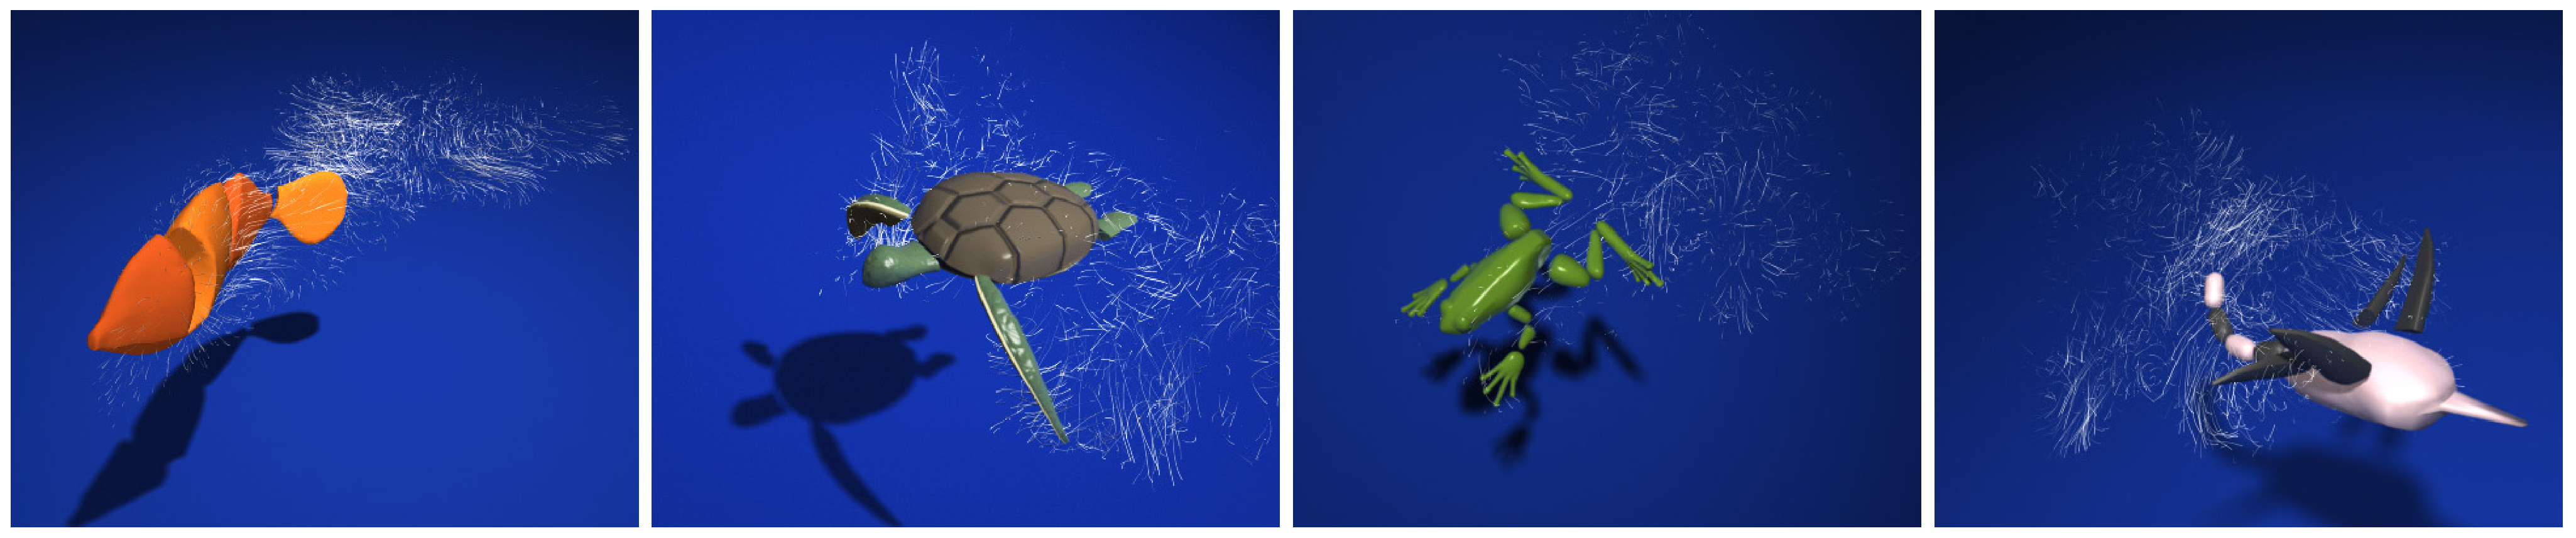
\includegraphics[width=\textwidth]{figures/teaserSwimming.eps}
  \caption{Aquatic creatures swim in a physically simulated hydrodynamic environment.}
  \label{fig:teaser1}
\end{figure}

The oceans cover over seventy percent of the area on our planet. They contain a wide variety of creatures that use swimming as their primary form of locomotion. Scientific studies show that the swimming gaits of the aquatic creatures are highly efficient compared to the man-made underwater vehicles. Studying their swimming motions could help us discover better propulsion mechanisms and design more efficient undersea vehicles to explore the largest uncharted territory on our planet. In Chapter 3, we apply numerical optimization to automatically discover the most energy efficient swimming gaits for given aquatic creatures in a physically-simulated hydrodynamic environment.

A main challenge in physical simulation is to model the complex interaction between two different types of dynamic systems, such as the two-way coupling between the fluid and a swimmer represented as an articulated rigid body system. We present an accurate physical simulator \cite{} that simultaneously solves the Navier-Stokes equations for fluids, the Lagrangian dynamics for an articulated rigid body and matches their accelerations at fluid-solid boundaries. The simulation results of swimming fish and eels show vortex trails that are in agreement with laboratory measurements.

Simulating fluid itself is hard; optimizing locomotion in a hydrodynamic environment is even more challenging. Previous methods have resorted to simplified fluid models. However, studies have shown that fish takes advantage of surrounding vortices, which are omitted in the simplified models, to provide energy boosts. Incorporating an accurate Navier-Stokes fluid model in the simulation presents new challenges in controller optimization: The optimization space is full of local minima due to the chaotic fluid behavior. Evaluating the gradient of the objective function is time-consuming. We demonstrate that sampling-based optimization algorithms are effective tools to overcome these challenges. This approach found efficient swimming motions that are comparable to those of real-world animals (Figure \ref{fig:teaser1}). 

\subsection{Locomotion for Soft Body Characters}

\begin{figure}[!h]
  \centering
    
\includegraphics[width=\textwidth]{figures/teaserSoftBody.eps}
  \caption{Soft body characters perform different forms of locomotion.}
  \label{fig:teaser2}
\end{figure}

While most research in character animation and robotics focus on characters that are made exclusively from rigid parts, we have seen an increasingly amount of efforts in the last few years to develop soft body robots \cite{}. While these research demonstrates a huge potential of soft body robots and their broad applications, it demands a new set of computational tools to study and to synthesize motions for soft body characters.

To model soft body characters, we not only need to simulate the passive dynamics of deformation, but also the actuation of muscles. In Chapter 4, we present a new mathematical model for artificial muscles that are motivated by the muscle structures of soft body animals in nature. Similar to real muscles, these artificial ones are arranged in groups and only allowed to contract. Complex movements need to be accomplished by the coordinated contraction of multiple muscle groups. We develop a finite element method with this muscle model to simulate soft body animals.

Optimizing controllers in the presence of discontinuous contact forces is a long-standing problem. Controlling locomotion for soft body characters (Figure \ref{fig:teaser2}) exacerbates the difficulty. The deformation of the body constantly changes the contact configuration between the character and the ground. A common practice is to separate contact planning and controller optimization. We identify that this simplification eliminates effective control strategies, and this causes the soft body character to lose balance. We derive an elegant solution to this problem that combines contact planning with controller optimization. We formulate a quadratic program with complementarity conditions (QPCC) and develop an efficient solver for QPCC problems derived from locomotion control with contacts. As a result, effective control strategies emerge automatically from the QPCC solution.

\subsection{Locomotion with Mechanical Devices}

\begin{figure}[!h]
  \centering
    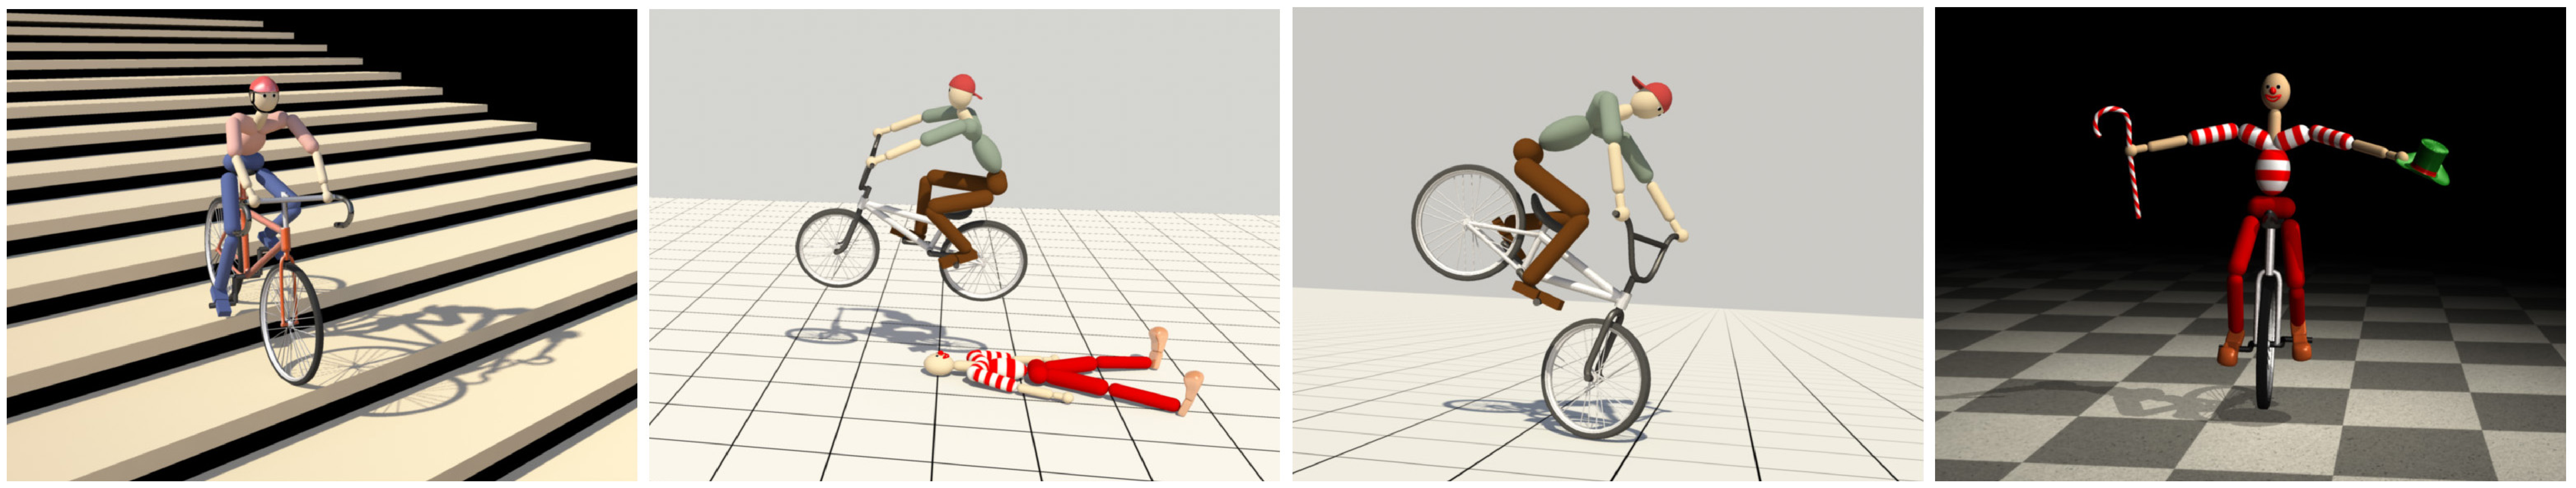
\includegraphics[width=\textwidth]{figures/teaserBicycle.eps}
  \caption{A human character performs stunts on a road bike, a BMX bike and a unicycle.}
  \label{fig:teaser3}
\end{figure}

Human has invented numerous mechanical tools to ease our life. Robots in the future can work much more efficiently if they can take advantage of these existing tools. Instead of manually programing the robots to master each tool, we hope that they can learn how to use them autonomously. Learning to ride a bicycle is an excellent case study. The bicycle, which has greatly boosted the efficiency of locomotion, was voted as the best invention since the 19th century. Even though the dynamics of bicycles is relatively well-understood, riding a bicycle is challenging due to the inherently unstable dynamics. In Chapter 5, we present a machine learning algorithm that allows a virtual character to learn to ride a bicycle in a physically simulated environment. 

In addition to the basic maneuvers, we hope that the character can learn more challenging but visually spectacular stunts (Figure \ref{fig:teaser3}). Performing stunts requires fast reaction, precise control and years of practice. This challenges the best human riders, let alone a machine learning algorithm. When we design the policy search algorithm, we find that the widely-used assumption of a predetermined controller parameterization severely limits the search space. It leaves the hard work to the user to design a good parameterization. We decide that optimizing the parameterization automatically is equally important as optimizing the parameters. Our algorithm evolves both the policy parameterization and the parameters simultaneously. This significantly improves the quality of the resulting controllers. Eventually, our simulated characters learn to perform a wide variety of bicycle stunts within hours, which is even faster than the best human stunt bikers.

\subsection{Locomotion Controller Transfer from Virtual to Real World}

Above three works demonstrate that with the powerful computational tools for character animation, natural, agile and robust motions can be synthesized efficiently and autonomously. However, creating lifelike robots is still an extremely challenging, trial-and-error process that is restricted to experts. The fast evolution of 3D printing technology will soon trigger a shift in the robotics industry from mass production to personalized design and fabrication, which will result in an immediate need for a faster, cheaper and more intuitive way to design robotic controllers. The computational tools we developed can potentially automate and streamline the process if we can transfer the controllers from the virtual simulation to the real world.

Transfering controllers optimized in a simulation onto a real robot is a non-trivial task. An optimal controller that works in a state-of-the-art simulation often fails in a real environment. This is known as the \emph{Reality Gap} \cite{}. This gap is caused by various simplifications in the simulation, including inaccurate physical model, unmodeled actuator dynamics, assumptions of perfect sensing and zero latency. In Chapter 6, we investigate some of these simplifications and present a general framework of simulation calibration. Simulation calibration optimizes simulation parameters to minimize the discrepancy between the data collected from real experiments on the robot and that generated in the simulation. After calibration, the simulation becomes more faithful to the real-world dynamics. Controllers that are designed with the improved simulator can work in both the virtual and the real world. 

\section{Contributions}

The computational tools presented in this dissertation provide several contributions to the communities of character animation and robotics. These contributions are as follows.

\paragraph{A stable simulation of two-way coupling between fluids and articulated rigid bodies.} We present a novel swimming simulator that can simultaneously solve the dynamics of fluids, articulated rigid bodies and their two-way interactions. Compared to the traditional two-way coupling solver that alternates the fluid update and the rigid body update, our method is more numerically stable. We are able to use time steps of 33ms for all our experiments without any stability problem. Using larger time steps makes our simulation orders of magnitude faster than the alternating solver. As a result, we can discover a swimming gait within days of computation while using the traditional two-way coupling technique may take weeks.

\paragraph{A finite element simulation with a muscle model for soft body animals.} Based on the muscle structure of muscular hydrostat \cite{} in real soft body animals, we develop a muscle model for the simulated characters. Combined with the finite element method for the passive deformation of the body, it provides intuitive ways to control the character in a coordinated manner. The use of this muscle model reduces the dimensionality of the control problem and results in more natural-looking motions.

\paragraph{An QPCC solver for motion optimization with changing contacts.} Controlling locomotion with contacts is a long-standing problem in continuous optimization because changes of contact situation (static, sliding or breaking) can introduce discontinuities to the dynamics. A commonly-used technique is to separate contact planning and controller optimization. However, this could eliminate effective locomotion strategies. We solve this problem by formulating a quadratic program with complimentarity conditions (QPCC). We also develop an efficient solver for QPCC problems with contacts. This method can optimize both the contact situation and forces simultaneously. As a result, interesting and effective locomotion strategies emerge automatically from the QPCC solution.

\paragraph{A reinforcement learning algorithm that searches both the parametrization and the parameters of a policy.} We present the first reinforcement learning algorithm which demonstrate that extremely challenging locomotion tasks, such as bicycle stunts, can be learned efficiently in simulation. Most of the stunt actions are learned within one hour, which is even faster than the performance of best human stunt bikers. These results present a new benchmark for future research in reinforcement learning. The key to such an efficient learning algorithm is an evolutionary optimization that can search for the parametrization and the parameters of a control policy simultaneously. We believe that this reinforcement learning algorithm can be generalized to master other challenging locomotion tasks.


\chapter{Pro and Con}

At the period when these events took place, I had just returned
from a scientific research in the disagreeable territory
of Nebraska, in the United States.  In virtue of my office
as Assistant Professor in the Museum of Natural History in Paris,
the French Government had attached me to that expedition.
After six months in Nebraska, I arrived in New York towards
the end of March, laden with a precious collection.
My departure for France was fixed for the first days in May.
Meanwhile I was occupying myself in classifying my mineralogical,
botanical, and zoological riches, when the accident happened
to the Scotia.

I was perfectly up in the subject which was the question of the day.
How could I be otherwise?  I had read and reread all the American
and European papers without being any nearer a conclusion.
This mystery puzzled me.  Under the impossibility of forming
an opinion, I jumped from one extreme to the other.
That there really was something could not be doubted,
and the incredulous were invited to put their finger on the wound
of the Scotia.\cite{incollection-full}

\section{An added section}

On my arrival at New York the question was at its height.
The theory of the floating island, and the unapproachable sandbank,
supported by minds little competent to form a judgment, was abandoned.
And, indeed, unless this shoal had a machine in its stomach,
how could it change its position with such astonishing rapidity?

From the same cause, the idea of a floating hull of an enormous
wreck was given up.

\vskip 0.25in
\begin{table}%
 \caption[Add a table]{Add an extra table here. Chinese Menu.}
 \begin{center}
  \begin{tabular}{lp{4.4cm}p{4.4cm}}
                & \textbf{column A} & \textbf{column B} \\
  \textbf{hot}  & Kung Pao Chicken  & General Tso's Chicken \\
  \textbf{mild} & Moo Goo Gai Pan   & Sweet and Sour Pork
  \end{tabular}
  \label{tab:test1}
 \end{center}
\end{table}

There remained, then, only two possible solutions of the question,
which created two distinct parties:  on one side, those who were
for a monster of colossal strength; on the other, those who were
for a submarine vessel of enormous motive power.

\subsection{A subsection}

But this last theory, plausible as it was, could not stand against
inquiries made in both worlds.  That a private gentleman should have
such a machine at his command was not likely.  Where, when, and how
was it built? and how could its construction have been kept secret?
Certainly a Government might possess such a destructive machine.
And in these disastrous times, when the ingenuity of man has
multiplied the power of weapons of war, it was possible that,
without the knowledge of others, a State might try to work such
a formidable engine.

But the idea of a war machine fell before the declaration of Governments.
As public interest was in question, and transatlantic communications
suffered, their veracity could not be doubted.  But how admit that
the construction of this submarine boat had escaped the public eye?
For a private gentleman to keep the secret under such circumstances would
be very difficult, and for a State whose every act is persistently watched
by powerful rivals, certainly impossible.


Upon my arrival in New York several persons did me
the honour of consulting me on the phenomenon in question.
I had published in France a work in quarto, in two volumes,
entitled Mysteries of the Great Submarine Grounds.  This book,
highly approved of in the learned world, gained for me a special
reputation in this rather obscure branch of Natural History.
My advice was asked.  As long as I could deny the reality
of the fact, I confined myself to a decided negative.
But soon, finding myself driven into a corner, I was
obliged to explain myself point by point.  I discussed
the question in all its forms, politically and scientifically;
and I give here an extract from a carefully-studied article
which I published in the number of the 30th of April.
It ran as follows:

\section{Another added section}

``After examining one by one the different theories, rejecting all
other suggestions, it becomes necessary to admit the existence
of a marine animal of enormous power.

\begin{equation}
E=mc^2
\end{equation}

``The great depths of the ocean are entirely unknown to us.
Soundings cannot reach them.  What passes in those remote depths---what 
beings live, or can live, twelve or fifteen miles beneath
the surface of the waters---what is the organisation of these animals,
we can scarcely conjecture.  However, the solution of the problem
submitted to me may modify the form of the dilemma.  Either we do know
all the varieties of beings which people our planet, or we do not.
If we do NOT know them all---if Nature has still secrets in the deeps
for us, nothing is more conformable to reason than to admit the existence
of fishes, or cetaceans of other kinds, or even of new species,
of an organisation formed to inhabit the strata inaccessible to soundings,
and which an accident of some sort has brought at long intervals
to the upper level of the ocean.

``If, on the contrary, we DO know all living kinds, we must
necessarily seek for the animal in question amongst those marine
beings already classed; and, in that case, I should be disposed
to admit the existence of a gigantic narwhal.

``The common narwhal, or unicorn of the sea, often attains
a length of sixty feet.  Increase its size fivefold or tenfold,
give it strength proportionate to its size, lengthen its
destructive weapons, and you obtain the animal required.
It will have the proportions determined by the officers
of the Shannon, the instrument required by the perforation
of the Scotia, and the power necessary to pierce the hull
of the steamer.\cite{inproceedings-full}

``Indeed, the narwhal is armed with a sort of ivory sword,
a halberd, according to the expression of certain naturalists.
The principal tusk has the hardness of steel.  Some of these tusks
have been found buried in the bodies of whales, which the unicorn
always attacks with success.  Others have been drawn out,
not without trouble, from the bottoms of ships, which they
had pierced through and through, as a gimlet pierces a barrel.
The Museum of the Faculty of Medicine of Paris possesses one
of these defensive weapons, two yards and a quarter in length,
and fifteen inches in diameter at the base.

``Very well! suppose this weapon to be six times stronger and the animal
ten times more powerful; launch it at the rate of twenty miles an hour,
and you obtain a shock capable of producing the catastrophe required.
Until further information, therefore, I shall maintain it to be
a sea-unicorn of colossal dimensions, armed not with a halberd,
but with a real spur, as the armoured frigates, or the `rams' of war,
whose massiveness and motive power it would possess at the same time.
Thus may this puzzling phenomenon be explained, unless there be something over
and above all that one has ever conjectured, seen, perceived, or experienced;
which is just within the bounds of possibility.''

\section{The last added section}

These last words were cowardly on my part; but, up to a certain point,
I wished to shelter my dignity as professor, and not give
too much cause for laughter to the Americans, who laugh well
when they do laugh.  I reserved for myself a way of escape.
In effect, however, I admitted the existence of the ``monster.''
My article was warmly discussed, which procured it a high reputation.
It rallied round it a certain number of partisans.  The solution
it proposed gave, at least, full liberty to the imagination.
The human mind delights in grand conceptions of supernatural beings.
And the sea is precisely their best vehicle, the only medium
through which these giants (against which terrestrial animals,
such as elephants or rhinoceroses, are as nothing) can be produced
or developed.

The industrial and commercial papers treated the question chiefly from this
point of view.  The Shipping and Mercantile Gazette, the Lloyd's List,
the Packet-Boat, and the Maritime and Colonial Review, all papers devoted
to insurance companies which threatened to raise their rates of premium,
were unanimous on this point.  Public opinion had been pronounced.
The United States were the first in the field; and in New York they
made preparations for an expedition destined to pursue this narwhal.
A frigate of great speed, the Abraham Lincoln, was put in commission
as soon as possible.  The arsenals were opened to Commander Farragut,
who hastened the arming of his frigate; but, as it always happens,
the moment it was decided to pursue the monster, the monster did not appear.
For two months no one heard it spoken of.  No ship met with it.
It seemed as if this unicorn knew of the plots weaving around it.
It had been so much talked of, even through the Atlantic cable, that jesters
pretended that this slender fly had stopped a telegram on its passage and was
making the most of it.

So when the frigate had been armed for a long campaign, and provided with
formidable fishing apparatus, no one could tell what course to pursue.
Impatience grew apace, when, on the 2nd of July, they learned that a
steamer of the line of San Francisco, from California to Shanghai,
had seen the animal three weeks before in the North Pacific Ocean.
The excitement caused by this news was extreme.  The ship was revictualled
and well stocked with coal.

Three hours before the Abraham Lincoln left Brooklyn pier,
I received a letter worded as follows:

\begin{longquote}
To M. ARONNAX, Professor in the Museum of Paris, Fifth Avenue Hotel, New York.

SIR,--If you will consent to join the Abraham Lincoln
in this expedition, the Government of the United States
will with pleasure see France represented in the enterprise.
Commander Farragut has a cabin at your disposal.

Very cordially yours, J.B. HOBSON, Secretary of Marine.
\end{longquote}

\chapter{Locomotion in Hydrodynamic Environments}

\section{Motivation}

We live on a planet that is covered mostly by water, in which a wide variety of
creatures use swimming as their primary form of locomotion.  There are
an astonishing variety of body shapes and patterns of motion that are used
by swimmers across the animal kingdom.  Some of the many creature swimming
patterns from nature include using thrust from a tail, moving an elongated
body sinusoidally, using paddle-like motions of flippers, kicking with legs,
and gentle bird-like flapping of fins.  Our research goal is to develop a
general platform for finding efficient swimming motion for a given creature
body shape.  There are a number of application areas that can benefit from
realistic swimming simulation, including feature film
animation~\cite{stanton2003finding}, biological investigation of swimming
mechanics~\cite{kern2006simulations,shirgaonkar2008hydrodynamics},
locomotion of user-created creatures in video games~\cite{hecker2008real},
and the invention of new modes of propulsion for underwater
vehicles~\cite{barrett2002optimal}.

Today, most scientific models for swimming motion are customized to specific
species with predefined locomotion patterns
\cite{shirgaonkar2008hydrodynamics}. These models are
highly accurate but are difficult to generalize to a variety of creatures.
The existing 3D swimming animations, on the other hand, demonstrate a
lifelike underwater ecosystem with rich variety of creatures. However, their motions are typically animated
manually or based on simplified physical models. Having a generic set of
tools that can produce physically realistic aquatic motion for a wide array
of creatures is challenging and has not been shown in previous work.

At the heart of synthesizing realistic aquatic locomotion lies the
problems of simulation and control. Solving these two problems
simultaneously under hydrodynamics presents some unique
challenges. First, the relation between the movement of the aquatic
animal and the forces exerted by surrounding fluid is extremely
complex. Thus it is difficult to solve using an optimization approach. Any small
changes in undulation or flapping gait can result in drastically
different control strategies. In addition, the morphology of aquatic
animals is astonishingly diverse and results in fundamentally
different locomotion mechanisms. Designing control strategies based on
ad-hoc observation or careful tuning of parameters would be extraordinarily difficult to generalize to the vast biodiversity found in nature.

This chapter describes a complete system for controlling a wide variety of
aquatic animals in a simulated fluid environment. Our goal is a system
that balances between physical realism and generality. Given an aquatic
animal that is represented by an articulated rigid body system, our system
can automatically find the optimal locomotion in a
hydrodynamically-coupled environment. Our system does not require any
prior knowledge of the animal's behavior and minimizes the effort of
manually tuning the physical and control parameters.

The system consists of two main components: simulating motion and
optimizing control strategies. We simulate articulated rigid bodies
submerged in invisid, incompressible fluid governed by the Navier-Stokes
equations. The animal can exert torques to exercise each actuated
joint. Through accurate two-way coupling of the rigid bodies and the
fluid, the joint motion will lead to \emph{some} locomotion in the
fluid, but purposeful and balanced locomotion requires careful
coordination and synchronization among those actuated joints.  The
second component provides an automatic way to discover joint motion
that achieves a desired goal in locomotion (i.e. a joint motion that
yields the fastest or the most energy efficient locomotion).  We
employ an optimization technique called Covariance Matrix Adaptation
(CMA) to explore the domain of possible joint trajectories.

We evaluate our system by demonstrating optimized swimming gaits for a
wider variety of aquatic animals and swimming strategies, including
clownfish, eels, sea turtles, frogs, manta rays and some imaginary
creatures. In addition, we compare the swimming motion in a Navier-Stokes
fluid with motion in a simplified fluid. Our results show that these
motions can differ dramatically depending on which fluid model is used.

\section{Swimming Simulation}

We simulate fluids by solving the Navier-Stokes equations on a MAC grid
and we simulate the articulated rigid body using generalized coordinates.
We modify the projection step of the fluid solver to take into
consideration the dynamics of the articulated figure.

\subsection{Fluid Simulation}

We simulate fluid using the inviscid, incompressible fluid equations
(sometimes called the Euler equations):
\begin{displaymath}
 \nabla\cdot\mathbf{u}=0
\end{displaymath}
\begin{displaymath}
 \mathbf{u}_t=-(\mathbf{u}\cdot\nabla\mathbf{u})-\frac{1}{\rho}\nabla
 p+\mathbf{f}
\end{displaymath}
where $\mathbf{u}=(u,v,w)$ is the velocity of fluids, $p$ is the pressure,
$\rho$ is the density and $\mathbf{f}$ accounts for the external body
forces.  We do not include a viscous term because such effects are
negligable for the motion of the large animals in our examples.  If we
were studying swimming of millimeter sized creatures, however,
incorporating viscous effects would be mandatory.

The standard way to solve the above equations on a MAC grid can be described in following two steps. First, we calculate an intermediate velocity field $\mathbf{u}^*$ by only considering the convection $\mathbf{u}\cdot\nabla\mathbf{u}$ and the body force $\mathbf{f}$:
\begin{equation}
 \mathbf{u}^*=\textrm{SL}(\mathbf{u}^n,\Delta t)+\Delta t\mathbf{f}
\label{eq:sl}
\end{equation}
where $\mathbf{u}^n$ is the velocity at $n^{th}$ time step.
We use the Semi-Lagrangian method \cite{stam99stablefluids} to integrate the convection term and apply BFECC \cite{kim06advectionswith} to reduce the numerical dissipation.

Next, we solve the following Poisson equation with Neumann boundary conditions $\mathbf{u}\cdot\mathbf{n}=\mathbf{u}_{solid}\cdot\mathbf{n}$ at the solid boundary and Dirichlet
boundary conditions $p = 0$ at the free surface. Then we project the intermediate velocity field to ensure the incompressibility condition.
\begin{equation}
\label{eq:poissonEqu}
 \nabla^2 p=\frac{\rho}{\Delta t}\nabla\cdot\mathbf{u}^*
\end{equation}
\begin{equation}
\label{eq:projection}
 \mathbf{u}^{n+1}=\mathbf{u}^*-\frac{\Delta t}{\rho}\nabla p
\end{equation}
In this work, we modify the second step ((\ref{eq:poissonEqu}) and (\ref{eq:projection})) to take into account the interaction between the fluid and the articulated rigid bodies.

\subsection{Articulated Rigid Body Simulation}
\label{sec:articulatedSim}
In this section, we will describe the numerical techniques that we use to move the body parts of an articulated figure. Later, in Chapter \ref{sec:optimization}, we will describe the optimization technique that we use to discover efficient swimming gaits.

The dynamic equations of an articulated rigid body in generalized coordinates can be expressed as follows.
\begin{equation}
\label{eq:swimDynamics}
\mathbf{M}(\mathbf{q})\mathbf{\ddot{q}}+\mathbf{C}(\mathbf{q},\mathbf{\dot{q}})=\mathbf{\tau}_{int}+\mathbf{\tau}_{ext}
\end{equation}
where $\mathbf{q}$, $\mathbf{\dot{q}}$ and $\mathbf{\ddot{q}}$ are vectors of positions, velocities and accelerations of joint degrees of freedom respectively. $\mathbf{M}(\mathbf{q})$ is the mass matrix and $\mathbf{C}(\mathbf{q},\mathbf{\dot{q}})$ accounts for the Coriolis and Centrifugal force. $\mathbf{\tau}_{int}$ and $\mathbf{\tau}_{ext}$ are internal and external generalized forces.

Given the current state $\mathbf{q}^n$ and $\mathbf{\dot{q}}^n$, we can
evaluate $\mathbf{M}$ and $\mathbf{C}$ of (\ref{eq:swimDynamics}). For the
external forces $\mathbf{\tau}_{ext}$, we consider the
fluid pressure force. We make use of the modified PD controller of Tan et al. \cite{Tan11SPD} in order to calculate the internal force $\mathbf{\tau}_{int}$ that closely tracks a reference trajectory. Although the details of this method can be found in \cite{Tan11SPD}, we include an overview of this method below. The reference swimming trajectory is computed by an optimization
process described in Chapter \ref{sec:optimization}. Once we know both the external and
internal forces, we can solve the acceleration $\mathbf{\ddot{q}}^n$ and
advance to the next time step via explicit Euler integration.

\paragraph {Modified Proportional-Derivative Controller} In computer
animation, a PD servo (\ref{eq:pd2}) provides a simple framework to
compute control forces for tracking a kinematic state of a joint
trajectory:
\begin{equation}
\label{eq:pd2}
\tau^n=-k_p(q^n-\bar{q}^n)-k_d\dot{q}^n
\end{equation}
where $k_p$ and $k_d$ are the gain and damping coefficient. In general,
high gain PD servos result in small simulation time steps in order to
maintain stability.

The aquatic creatures in this work require high gain PD servos to track the desired swimming gait closely against strong fluid pressure. However, we cannot reduce the time step to accommodate stability due to the time-consuming fluid simulation. To achieve these two conflicting goals, large time steps and high gains, we modify the PD controller as follows. Instead of using the current state $q^n$ and $\dot{q}^n$ to compute the control force, we compute the control forces using the state at next time step $q^{n+1}$ and $\dot{q}^{n+1}$:
\begin{equation} \label{eq:pd3}
\tau^n=-k_p(q^{n+1}-\bar{q}^{n+1})-k_d\dot{q}^{n+1}
\end{equation}

eq. (\ref{eq:pd3}) can be linearized at $q^n$ and $\dot{q}^n$ as:
\begin{displaymath}
\tau^n=-k_p(q^n+\Delta t\dot{q}^n-\bar{q}^{n+1})-k_d(\dot{q}^n+\Delta t\ddot{q}^n)
\end{displaymath}

Applying the modified PD controller to the articulated rigid body simulation with multiple degrees of freedom, we solve the acceleration as
\begin{displaymath}
\label{eq:modifiedDynamics}
\mathbf{\ddot{q}}^n=(\mathbf{M}+\mathbf{K}_d\Delta t)^{-1}(-\mathbf{C}-\mathbf{K}_p(\mathbf{q}^n+\mathbf{\dot{q}}^n\Delta t-\bar{\mathbf{q}}^{n+1})-\mathbf{K}_d\mathbf{\dot{q}}^n+\mathbf{\tau}_{ext})
\end{displaymath}
where both $\mathbf{K}_p$ and $\mathbf{K}_d$ are diagonal matrices that indicate the gains and damping coefficients.

\subsection{Two-way Coupling Between Fluids and Articulated Rigid Bodies}
The two-way coupling between the incompressible fluid and the articulated figures should satisfy following three conditions.
\begin{enumerate}
\item The normal velocity at the interface between the fluids and the
articulated rigid bodies should agree with each other.
\item The motion of the articulated rigid body resulting from the fluid
pressure force must be consistent with the Lagrangian equations of motion.
\item The fluid should be incompressible.
\end{enumerate}

Two-way coupling is ensured by having the fluid exerting pressure forces
on the rigid bodies, while at the same time the motion of the rigid bodies
affects the pressure distribution of the fluid.

Our simultaneous two-way coupling technique is inspired by Klingner et al.
\cite{klingner2006mesh} since we both start from the acceleration at
cell faces.  Their method uses a tetrahedral mesh to represent the fluid,
and their rigid bodies are in Cartesian space.  Our simulator uses a
regular MAC grid and we couple this fluid with articulated figures that
are described in generalized coordinates.  Similar to Klingner et
al.~\cite{klingner2006mesh}, we split the coupling into two steps
(Figure~\ref{fig:graph}). In the first step, the two systems are solved
independently ignoring the pressure. The fluid solver calculates the
intermediate velocity field $\mathbf{u}^*$ using (\ref{eq:sl}). The articulated
rigid body solver determines the acceleration $\mathbf{\ddot{q}}$ without
external pressure forces and calculates the intermediate velocity
$\mathbf{\dot{q}}^*$.

\begin{figure}[t]
\centering
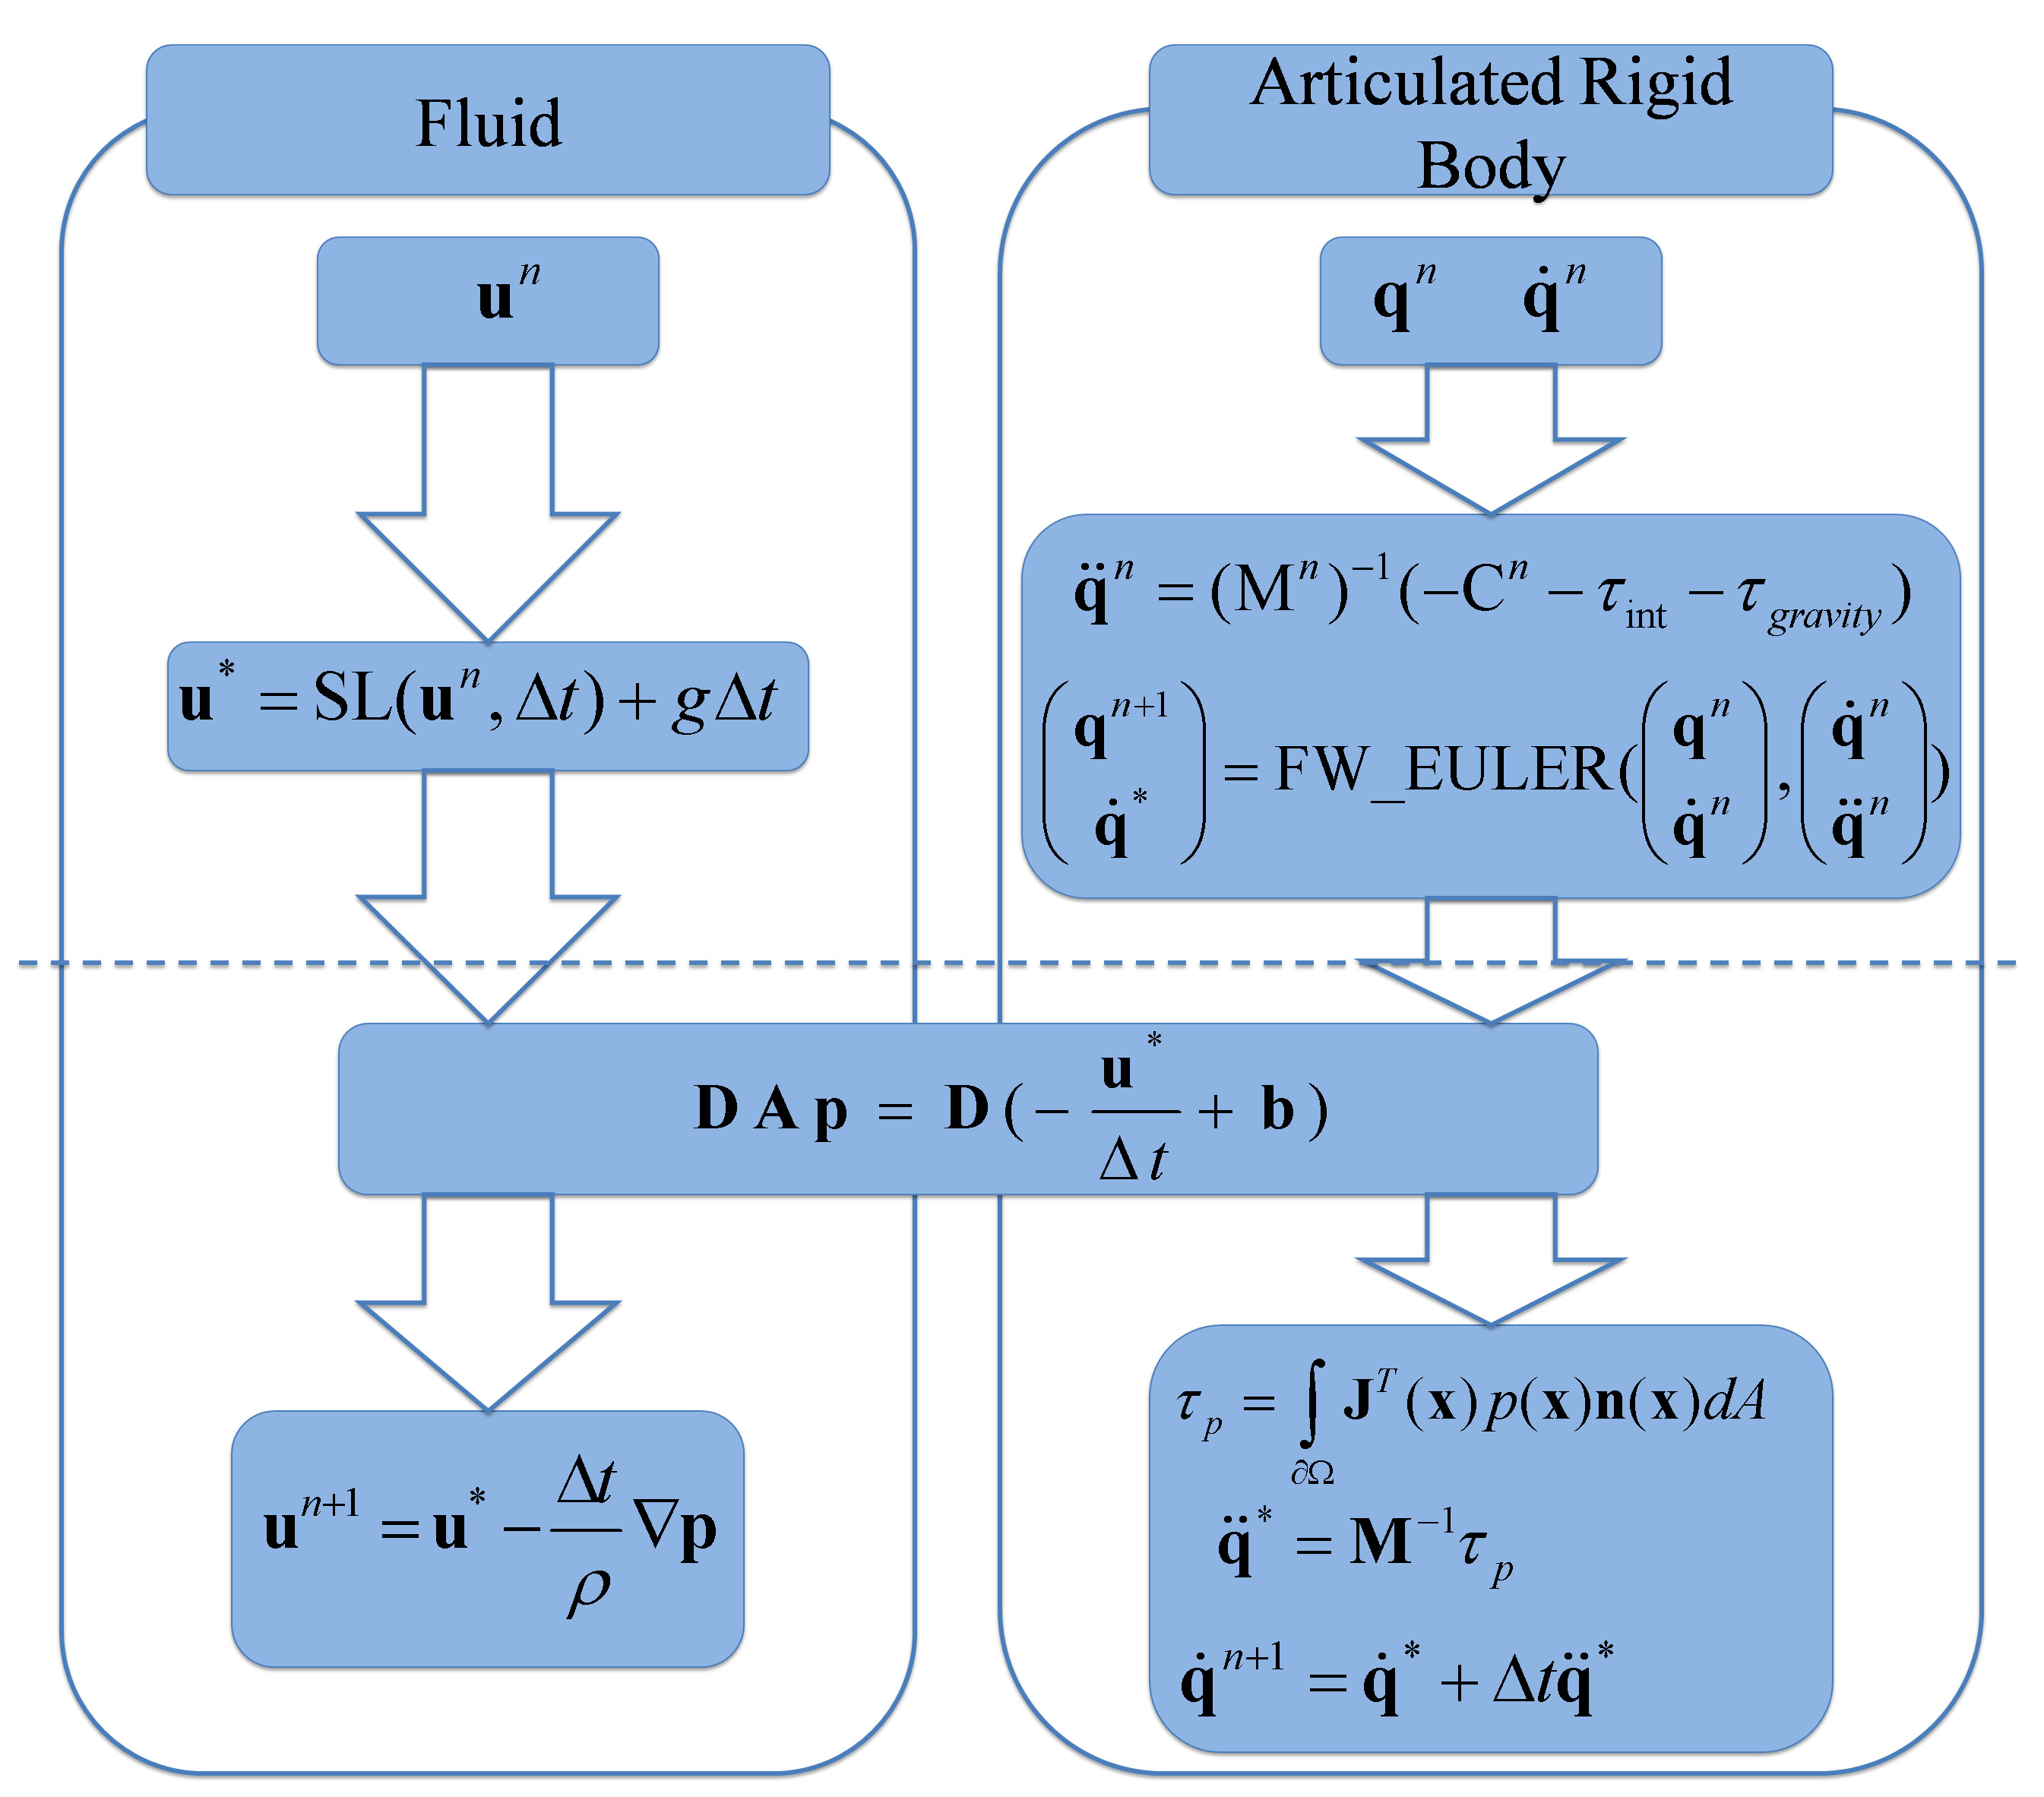
\includegraphics[width=3in]{figures/CouplingProcess.eps}
\caption{The computational steps for simultaneous coupling between fluids and articulated rigid bodies.}
\label{fig:graph}
\end{figure}

In the second step, we consider the motion of the two systems together so
that they will satisfy all above three conditions. We first voxelize the
body segments of the articulated figure (represented by water-tight
polygon meshes) onto the MAC grid and we mark those cells inside the body
segments as SOLID. For two-way coupling, we are particularly interested in
the faces between a SOLID cell and a FLUID cell (defined as \emph{coupled
faces}). The velocity at a coupled face can be expressed in generalized
coordinates by the Jacobian of the articulated rigid body and the joint
velocity:
\begin{displaymath}
\mathbf{u}^*_{solid}=\mathbf{J}\mathbf{\dot{q}}^*
\end{displaymath}
where $\mathbf{J}$ is the $3\times m$ ($m$ is the number of degrees of freedom) Jacobian matrix
\begin{displaymath}
\mathbf{J}=
\left( \begin{array}{cccc}
\frac{\partial x}{\partial q_1} & \frac{\partial x}{\partial q_2} & \ldots & \frac{\partial x}{\partial q_m} \\
\frac{\partial y}{\partial q_1} & \frac{\partial y}{\partial q_2} & \ldots & \frac{\partial y}{\partial q_m} \\
\frac{\partial z}{\partial q_1} & \frac{\partial z}{\partial q_2} & \ldots & \frac{\partial z}{\partial q_m}
\end{array} \right)
\end{displaymath}

Now consider the effect of the pressure field, which exerts forces and
applies accelerations along the face normals $\mathbf{n}$. If a face is
shared by two FLUID cells, the acceleration is
$\frac{1}{\rho}\nabla\mathbf{p}\cdot\mathbf{n}$. If a face is shared by a
FLUID cell and a SOLID cell (a coupled face), we need to take into account
all the pressure values surrounding the articulated rigid body. We first
construct a $k\times n$ selection matrix $\mathbf{S}$ to pick out of $\mathbf{p}$ the
pressures at the coupled faces, where $k$ is the number
of the coupled faces and $n$ is the number of FLUID cells. Thus the vector
$\mathbf{Sp}$ constains all the pressure values surrounding the
articulated rigid body. Each element $p_i$ of $\mathbf{Sp}$ contributes a
pressure force $(\Delta x)^2p_i\mathbf{n}_i$ to the articulated rigid
body, which we transform to the generalized coordinate:
\begin{displaymath}
\mathbf{\tau}_{p_i}=\mathbf{J}_i^T(\Delta x)^2p_i\mathbf{n}_i
\end{displaymath}
The total generalized force exerted by the fluid pressure on the articulated rigid body is
\begin{displaymath}
\mathbf{\tau}_p=(\Delta x)^2\hat{\mathbf{J}}\mathbf{Sp}
\end{displaymath}
where $\hat{\mathbf{J}}=[\mathbf{J}_0^T\mathbf{n}_0~~~~~\ldots~~~~~\mathbf{J}_k^T\mathbf{n}_k]$. The pressure force results in the acceleration in generalized coordinates
\begin{displaymath}
\mathbf{\mathbf{\ddot{q}}_{p}}=\mathbf{M}^{-1}\mathbf{\tau}_{p}
\end{displaymath}
We transform the acceleration back to Cartesian space, and the magnitude of the acceleration at the coupled face is
\begin{displaymath}
a=\mathbf{n}^T(\mathbf{J\ddot{q}_p}+\mathbf{\dot{J}\dot{q}}^*)
\end{displaymath}
The second term $\mathbf{\dot{J}\dot{q}}^*$ comes from the fact that the Jacobian matrix changes over time. Stacking the accelerations at the coupled faces into a vector, we have
\begin{equation}
\label{eq:acceleration}
\mathbf{a}=(\Delta x)^2\hat{\mathbf{J}}^T\mathbf{M}^{-1}\hat{\mathbf{J}}\mathbf{Sp}+\dot{\hat{\mathbf{J}}}^T\mathbf{\dot{q}}^*
\end{equation}
where
$\dot{\hat{\mathbf{J}}}=[\mathbf{\dot{J}}_0^T\mathbf{n}_0~~~~~\ldots~~~~~\mathbf{\dot{J}}_k^T\mathbf{n}_k]$.

Since the velocity field should be divergence free at the beginning of the next time step,
\begin{equation}
\label{eq:divFree}
\nabla\cdot\mathbf{u}^{n+1}=\nabla\cdot(\mathbf{u}^*+\Delta t\mathbf{a})=0
\end{equation}
the accelerations due to the pressure must satisfy the following equation.
\begin{displaymath}
\nabla\cdot\mathbf{a}=-\frac{1}{\Delta t}\nabla\cdot\mathbf{u}^*
\end{displaymath}
Putting everything together, we reach the final linear system:
\begin{equation}
\label{eq:pressureEqu}
\mathbf{D}\mathbf{A}\mathbf{p}=\mathbf{D}(-\frac{\mathbf{u}^*}{\Delta t}+\mathbf{b})
\end{equation}
\begin{displaymath}
\begin{array}{ll}
\mathbf{A} = & \left\{ \begin{array}{ll}
\frac{1}{\rho}\mathbf{G} & \textrm{faces shared by two FLUID cells}\\
(\Delta x)^2\hat{\mathbf{J}}^T\mathbf{M}^{-1}\hat{\mathbf{J}}\mathbf{S} & \textrm{coupled faces}
\end{array} \right. \\
\mathbf{b} = & \left\{ \begin{array}{ll}
\mathbf{0} & \textrm{~~~~~~~~~~~~~~~faces shared by two FLUID cells} \\
-\dot{\hat{\mathbf{J}}}^T\mathbf{\dot{q}}^* & \textrm{~~~~~~~~~~~~~~~coupled faces}
\end{array} \right.
\end{array}
\end{displaymath}
where $\mathbf{D}$ and $\mathbf{G}$ are the discretization of the divergence and gradient operators on a MAC grid.

We construct a system of linear equations (\ref{eq:pressureEqu}) for the
pressure field, which considers all of the three conditions to be
satisfied by the coupled system. The fluid and solid velocity agrees at
the interface (condition 1) because the velocity defined at the coupled
faces are shared by the fluid and the articulated body. The movement of
the articulated rigid body under the fluid pressure satisfies the equation
of motion (condition 2) because (\ref{eq:acceleration}) is derived from
the dynamics (\ref{eq:swimDynamics}). The fluid is incompressible
(condition 3) because we enforce the divergence free condition by
(\ref{eq:divFree}). The linear system is of the same size as the
discretized Poisson equation (\ref{eq:poissonEqu}) in a typical fluid
simulation.  The main difference is that the rows correpsonding to the
cells adjacent to the SOLID cells have more non-zero entries. Furthermore,
it is also symmetric positive definite, which allows the use of fast
solvers such as the Preconditioned Conjugate Gradient method. After
solving the pressure field, we project the velocity field to make it divergence free
using (\ref{eq:projection}) and update the articulated rigid body by
considering the pressure forces.

\section{Swimming Gait Optimization}
\label{sec:optimization}

We have described the two-way interaction between fluids and an articulated rigid body system. In particular, Chapter \ref{sec:articulatedSim} describes how we move the body parts using torques and how we compute the torques for a given reference gait. In this section, we describe an algorithm to automatically design optimal controllers for an active articulated
rigid body systems that is moving in a hydrodynamic environment.  Our
method generates physically realistic strokes based on the swimming
efficiency of the stroke.

\subsection{Swimming Gait Representation}

Given the geometric and physical properties of an articulated rigid body
system, we formulate an optimization to solve for the reference trajectory
of PD controller at each actuated joint, $q_i$.  We want to use a
compact representation for the reference trajectory because
incorporating a fluid simulation into the optimization is computational
intensive. Because aquatic locomotion is typically cyclic, we parameterize
the reference trajectory as periodic cycles in generalized coordinates.
\begin{displaymath}
q_i(t)=A_i\sin(\frac{2\pi t}{T_i}+\phi_i)+C_i
\end{displaymath}
where $A_i, T_i, \phi_i$ and $C_i$ are the amplitude, period, phase and
offset of a sine function. Using this parameterization, each reference
trajectory $q_i(t)$ is parameterized by four values.  In most cases we
just optimize over two parameters, amplitude and phase, and leave the
period and offset fixed.

\subsection{Objective Function}
\label{sec:swimmingObj}
The objective function in our optimization tries to balance between
efficiency and energy expenditure of the swimming gait; the creature
should move as fast as possible in the desired direction without using too
much energy. Furthermore, the creature should try to avoid self-collisions
and remain within the joint limits. In practice, the choice of objective
function can vary by creatures, fluid conditions, or the user's
application. Here we choose a simple objective function to find natural
swimming motion:
\begin{equation}
\label{eq:objFunc}
E=-E_{distance}+w_1E_{deviation}+w_2E_{energy}+w_3E_{collision}
\end{equation}
where $E_{distance}$ measures the change of the creature's root position $\Delta\mathbf{p}$ along a specified direction $\mathbf{d}$ from time 0 to time $t_f$:
\begin{displaymath}
E_{distance}=\mathbf{d}^T(\Delta\mathbf{p})
\end{displaymath}

$E_{deviation}$ measures the deviation from the specified direction and the initial orientation.
\begin{displaymath}
E_{deviation}=||\Delta\mathbf{p}-\mathbf{d}^T(\Delta\mathbf{p})\mathbf{d}|| + ||\Delta\mathbf{\alpha}||
\end{displaymath}
where $\Delta\mathbf{\alpha}$ stands for the change of root orientation in $t_f$, expressed using the exponential map. Since we're optimizing the gait of straight swimming, we penalize any orientation changes. We choose the weight $w_1=0.2$ for all the examples.


$E_{energy}$ penalizes the energy expenditure of the swimming gait.  We
calculate the work done by the actuated joints over the duration of the
swimming gait:
\begin{displaymath}
E_{energy}=\int_{0}^{t_f}\sum_i\tau_i\dot{q}_idt
\end{displaymath}

Instead of penalizing energy expenditure linearly, we modulate $E_{energy}$ with a discontinuous function represented as the objective weight $w_2$.  Instead of constantly trying to avoid using any energy, this modulation allows the creature to freely consume a certain amount of energy, while avoiding excessive use of torques.
\begin {displaymath}
\begin{array}{ll}
w_2 = & \left\{ \begin{array}{ll}
0 & \textrm{if }E_{energy} < E_{energyBound}\\
1 & \textrm{otherwise}
\end{array} \right. \\
\end{array}
\end {displaymath}
where $E_{energyBound}$ is a user specified parameter.

$E_{collision}$ penalizes self-intersection. We detect self-intersection
and calculate the overlapping volumes using a fast approximate method.
We first voxelize the articulated rigid body using a fine grid (the
typical grid resolution is about $100^3$). If a cell is inside a body
link, we increment the counter for that cell. At each time step, we sum up
all the cells with counter number larger than one and multiply by the
cell volume to approximate the overlapping volume.
\begin{displaymath}
E_{collision}=\int_{0} ^{t_f}V_{overlap}dt
\end{displaymath}
where $w_3$ is chosen to be $500$ for all the examples.

\subsection{Optimization}
\label{sec:CMAOptimization}
\newtext{Solving the above optimization presents unique challenges. First,
  we do not have good initial guesses for different swimming patterns of a wide variety of
  animals with distinctive morphologies. Second, evaluating gradient is expensive because each evaluation needs to simulate the fluid. Last but not least,} our objective function is discontinuous and prone to local minima due to sub-optimal swimming gaits, collision penalties, and the modulation of the energy penalty term. \newtext{For the above reasons, it is difficult to apply traditional continuous optimization algorithms that perform gradient-guided ``local'' search near the initial guesses.} To solve these problems, we perform gait optimization using Covariance Matrix
Adaptation (CMA).  \newtext{CMA is a stochastic sample-based optimization algorithm. It does not rely on good initializations and it does not need to compute gradient. More importantly, CMA is a ``global'' search algorithm that can explore multiple local minima. Although there is no guarantee that CMA will converge at the global minimum, in practice, we observe that it often finds good local minima in moderately high dimensional control spaces (\eg 20-30 dimensions). I believe that other sample-based optimization algorithms, such as Particle Swarm Optimization \cite{Kennedy:1995}, may also work well for this problem, although they are not tested in our implementation.}

CMA is based on evaluating the objective function for a
given population of samples over the parameter space (in our case the
joint trajectories).  Some fraction of the best samples are then used to
update the mean and a covariance matrix that determines the distribution
of samples that are evaluated in the next generation.  More details
of the CMA method can be found in~\cite{hansen2004evaluating}.

For each CMA sample, if it violates the user specified joint limits we
simply discard it and select another sample. Because the joint limit test
takes very little computation time, discarding infeasible samples at this
stage is more ``economical'' than investing major computation effort
on them but assigning them a near-zero weight at the end. Once a sample is
accepted, we simulate the motion by applying the sampled swimming gait and
evaluate the resulting motion using the objective function. To speed up
CMA for solving such high-dimensional problems, we include two heuristics
in our implementation for some examples. First, we utilize symmetry for
some of our articulated figures: When a creature's body shape is symmetric, often its gait is also symmetric. In such cases, half of the optimization variables are enough to characterize the gait of the whole body because we mirror them to the other half of the body. This assumption is applied to reduce the required computational time, but it is not necessary.
Second, for creatures that have more
independent appendages, we separate the degrees of freedom in groups and
progressively improve the solution by optimizing each group. For example,
we assign the forelimbs and hindlimbs of a frog into two separate groups.
During the optimization, we first search for the swimming gait for the
hindlimbs while freezing the motions of the forelimbs. We then search for
the swimming gait of the forelimbs with the optimal hindlimb motions that we
already found.

\section{Path Following}

\begin{figure}[!b]
\centering
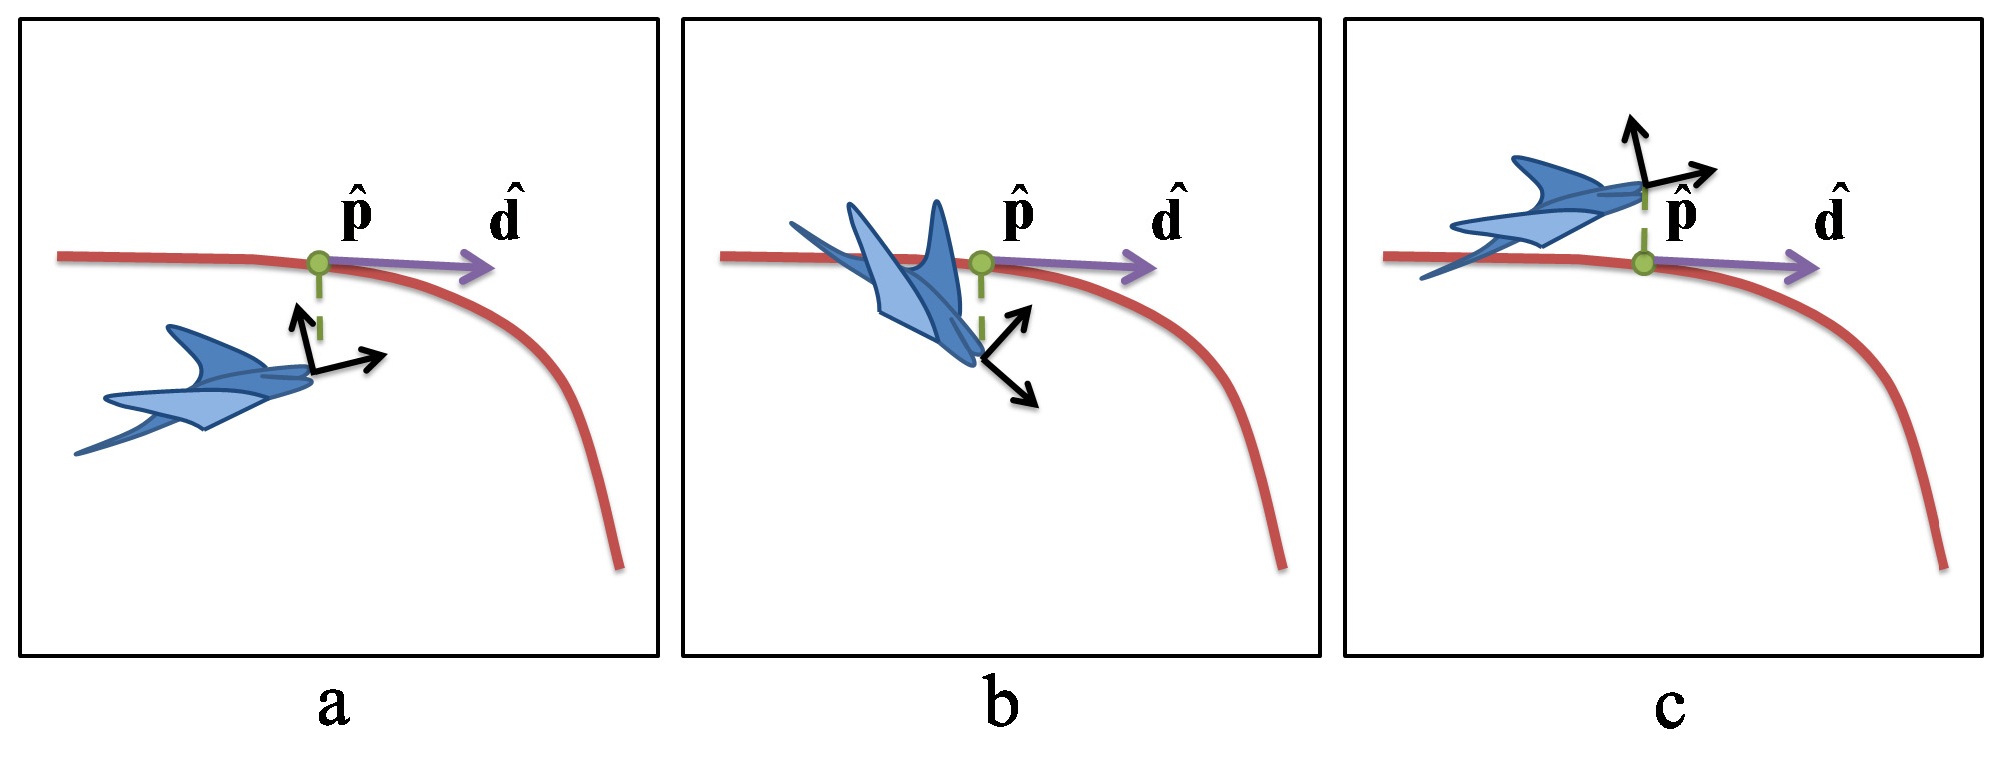
\includegraphics[width=3.2in]{figures/pathCase.eps}
\caption{Three different situations that determine if the creature chooses a ``swim straight'', ``pitch up'' or ``pitch down'' maneuver.}
\label{fig:pathCases}
\end{figure}

In addition to forward thrust, aquatic creatures also employ very
efficient turning maneuvers, such as pitching up and down or turning left
and right. The optimization technique described in Chapter
\ref{sec:optimization} can be modified to learn various
maneuvers. Once the aquatic creature builds a repertoire of swimming
maneuvers, we can combine different maneuvers to achieve a high-level
task such as path following.

First, we add another term to $E_{distance}$ in (\ref{eq:objFunc}) to maximize the turning angle towards the desired direction:
\begin{displaymath}
E_{distance}=\mathbf{d}^T(\Delta \mathbf{p})+\mathbf{r}^T(\Delta\mathbf{\alpha})
\end{displaymath}
where $\mathbf{r}$ is the desired axis of rotation. We set the desired swimming direction $\mathbf{d}$ half way from the current facing direction towards the turning direction. We also change $E_{deviation}$ to penalize the undesired orientation changes.
\begin{displaymath}
E_{deviation} = ||\Delta\mathbf{p}-\mathbf{d}^T(\Delta\mathbf{p})\mathbf{d}|| + ||\Delta\mathbf{\alpha}-\mathbf{r}^T(\Delta\mathbf{\alpha})\mathbf{r}||
\end{displaymath}
We solve the above optimization using the CMA method in the same way as described in Chapter \ref{sec:CMAOptimization}.

Once different maneuvers have been learned, we apply a simple heuristic to
decide which maneuver to choose to follow the path. At the beginning of
each cycle of the motion, we find the nearest point $\mathbf{p}$ on the
path to the root of the articulated figure and transform $\mathbf{p}$ and
its tangential direction $\mathbf{d}$ to the root coordinate system. We
denote the transformed position and direction as $\hat{\mathbf{p}}$ and
$\hat{\mathbf{d}}$. Without loss of generality, let's consider a one
dimensional example. $\hat{p}_z$ is the z-component of $\hat{\mathbf{p}}$,
which means the point is above or beneath the root of the articulated
figure. Similarly, $\hat{d}_z$ indicates the path is going upwards or
downwards relative to the root orientation. We choose the different
maneuvers based on the following rules.

\begin{figure}[!t]
\centering

\includegraphics[width=3.2in]{figures/skels.eps}
\caption{The joint configurations of the frog, the manta ray and the alien.}
\label{fig:skels}
\end{figure}

\begin{figure}[!t]
\centering
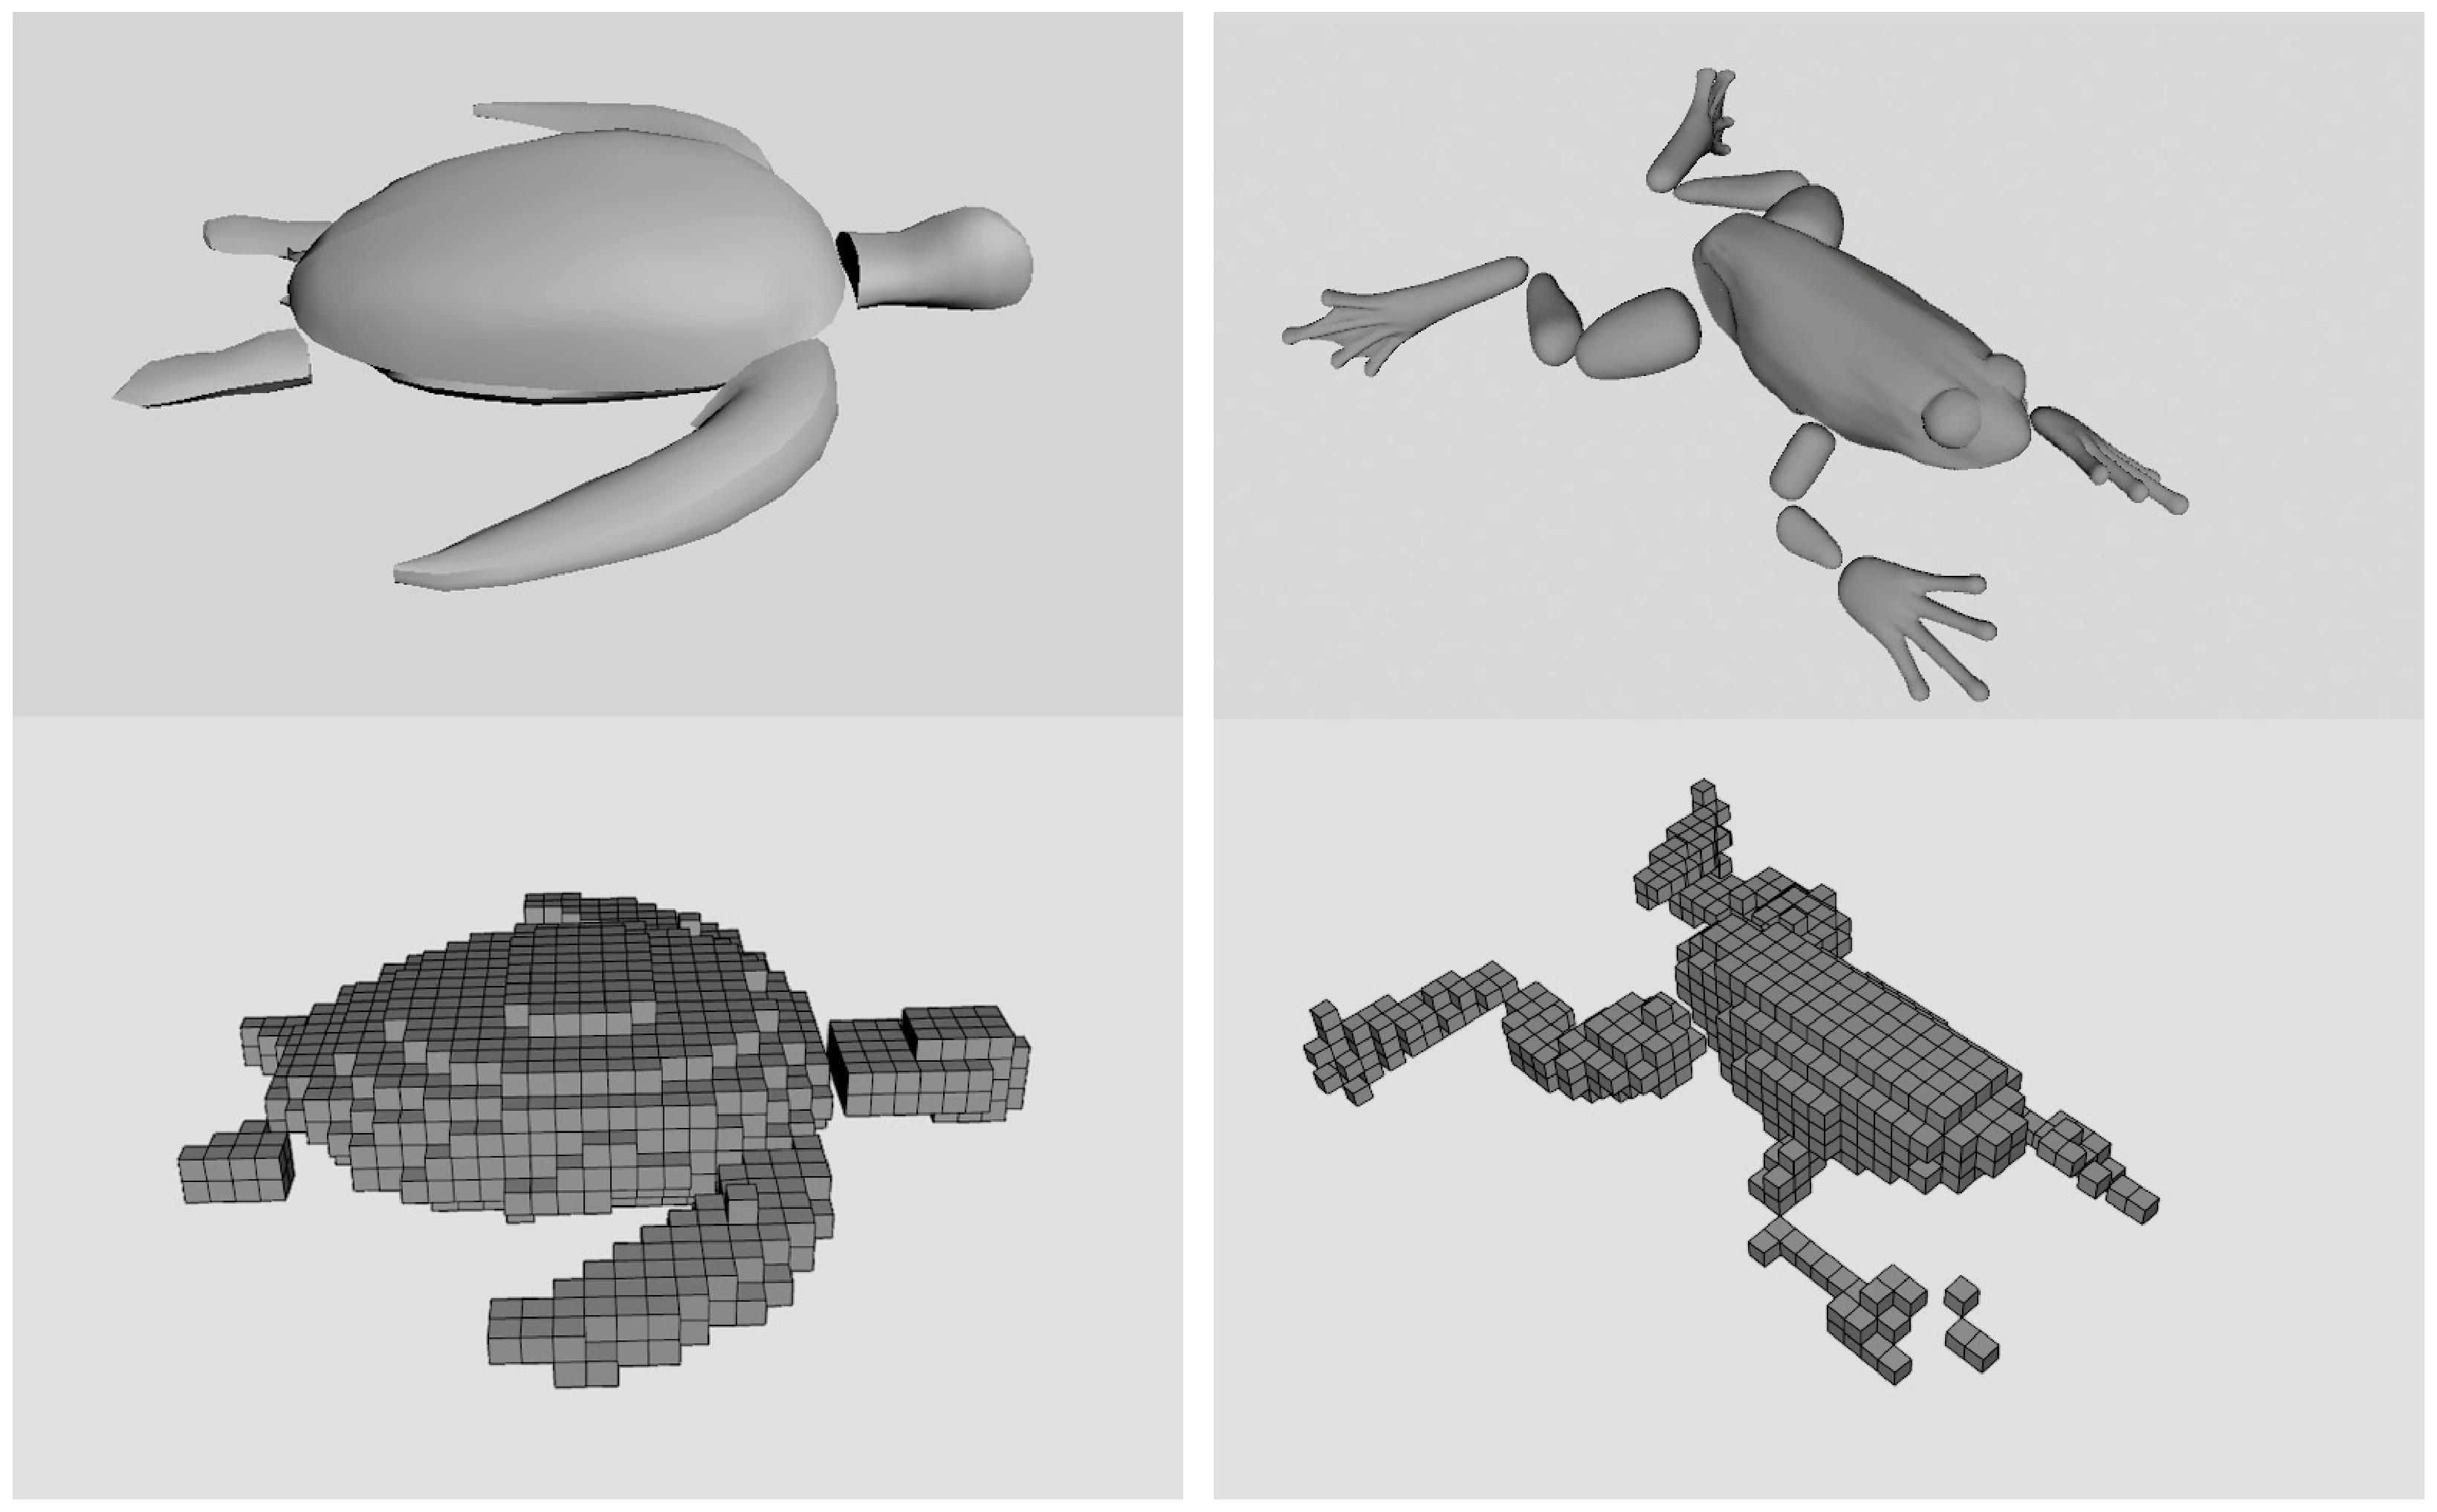
\includegraphics[width=3.2in]{figures/grid1.eps}
\caption{The voxelized representations of the turtle and the frog. The input shapes of the articulated creatures are represented by water-tight polygon meshes. We voxelize these body shapes onto the simulation grid each time step to simulate the two-way coupling between the fluid and the creature.}
\label{fig:grid}
\end{figure}


\begin{displaymath}
\textrm{Maneuver}=\left\{\begin{array}{ll}
\textrm{Go Straight} & \textrm{if } (\hat{p}_z \geq \epsilon \textrm{ and }\hat{d}_z \leq -\epsilon)\\
                     & \textrm{or } ( \hat{p}_z \leq -\epsilon \textrm{ and } \hat{d}_z \geq \epsilon)\\
\textrm{Pitch Up} & \textrm{if } \hat{p}_z > \epsilon \textrm{ and } \hat{d}_z > \epsilon\\
\textrm{Pitch Down} & \textrm{if }\hat{p}_z < -\epsilon \textrm{ and } \hat{d}_z < -\epsilon
\end{array}\right.
\end{displaymath}
where $\epsilon$ is a small positive value to prevent the articulated
figure from repeatedly choosing alternating turning maneuvers due to small
deviations from the path. The first case indicates that the nearest point
on the path is above/below the articulated figure while the direction of
the path is going downwards/upwards. In other words, the articulated
figure is swimming towards the path (Figure~\ref{fig:pathCases}a). We
choose the action ``swim straight'' in this situation. On the other hand,
the second and third cases indicate the articulated figure is swimming
away from the path (Figure~\ref{fig:pathCases}b and \ref{fig:pathCases}c)
and we choose ``pitch up'' or ``pitch down'' accordingly.

\section{Results}


We implemented our method using C++ and ran CMA on a cluster with a
maximum of 100 iterations and with a population size of 16 for 2D and 31 for 3D
examples. Each CMA sample evaluates the objective function by simulating
two cycles of swimming motions. The optimization took from several hours
to two days, depending on the model and the grid resolution. After we
found the swimming gait, we ran the swimming simulation on a 2.26GHz CPU
with a single core.  All of the data for our swimming examples are
summarized in Table~\ref{table:simData}. In most of the cases, we use two
optimization variables, amplitude and phase, for each degree of freedom.
We set the period to one second and the offset to zero. When training the
turning gaits, we included the offset in the optimization variables. For the
accordian example, the degrees of freedom are interdependent and there is
no phase shift among the different degrees of freedom. Thus one
optimization variable is enough to characterize its motion. We also
exploited the strong symmetry in geometry for some creatures, such as
turtles and frogs, to halve the optimization dimensions. We illustrate the
joint configurations for some creatures in Figure~\ref{fig:skels} and the voxelized representations of creatures in Figure~\ref{fig:grid}.

\begin{table}
  \centering
   \caption{Parameters and performance of examples. Num DOFs is the number of degrees of freedom for the articulated rigid body. Opt Dims is the number of optimization variables. Sim Res is the grid resolution for the simulation and Sim Time is the average simulation time per frame.}
\begin{tabular}{|c|c|c|c|c|}
\hline
Examples & Num & Opt  & Sim  & Sim\\
         & DOFs & Dims & Res & Time \\
 \hline
accordian & 10 & 1 &  $120\times 80$           & 1.37s\\
eel(2D)   & 4  & 8 &  $128 \times 64$         &  0.64s \\
turtle(2D)& 4  & 4 & $64\times 64$           & 0.34s \\
fish      & 3  & 6  & $64\times 32\times 32$  & 1.45s\\
eel(3D)   & 6  & 12 &  $64\times 32\times 32$ & 1.31s\\
manta-ray & 14 & 21 &  $64\times 32\times 32$ & 10.92s\\
turtle(3D)& 10 & 10 &  $64\times 32\times 32$ & 11.29s\\
frog      & 18 & 18 &  $96\times 64\times 48$ & 12.79s\\
alien     & 16 & 24 &  $96\times 36\times 24$ & 10.75s\\

\hline
 \end{tabular}
 \label{table:simData}
 \end{table}

In our implementation, we made three simplifications to reduce the
simulation cost. 1) Instead of using a large computational domain to cover
the whole space that the creature might swim to, we use a smaller domain
that is about two to four times larger in each dimension than the
creature's bounding box. This domain moves with the creature when the
creature approaches a boundary. 2) At the boundary of the computional
domain, we impose the Dirichlet boundary condition $p=0$ so that the fluid
outside the domain is free to flow in and vice versa. 3) Since the density
of most aquatic creatures is similar to that of the fluid, we ignore the force of gravity in our simulator.

We describe the results of our swimming optimization method.  Please see the video\footnote{https://dl.dropboxusercontent.com/u/36899427/articulatedswimmingcreatures.mp4} to observe the swimming
animations.  To visualize the fluid flow, we draw \emph{particles traces},
which show the trajectory of massless particles inside the fluid in a
short period of time (15 frames). We modulate the transparency of the
particle traces in 3D examples according to the magnitude of the vorticity
in order to focus attention on the visually interesting regions of the
flow.  In 2D examples, we colored the traces to indicate the directions of
the vortices.


There are many body shapes and styles of locomotion for fish, and our
first set of results investigates several of these.  Figure~\ref{fig:fish}
shows a four-segment model of a fish, modelled after the body shape of the
clownfish.  We used CMA to optimize for efficient forward motion, and snapshots of the resulting motion are given in the figure.  Note that the
forward body flexes just a little, with the majority of the motion near
the tail, which is in good agreement for the style of motion known as the
carangiform mode~\cite{lindsey1978form}.  Using the same objective
function, we optimized a seven-segment figure that was designed to mimic
an eel body.  Figure~\ref{fig:eel} shows that the resulting motion is that
of a travelling wave along the body of the creature, as is typical of real
eel swimming (anguiliform mode).  Note that the wake of our eel has two
separate trails of vortices that are shed from the tip of the tail, as has
been observed in lab studies of eels~\cite{tytell2004hydrodynamics}. We show in Figure~\ref{fig:eel2D} that a different wake structure appears when an eel swims in a 2D fluid environment, that of a single vortex street. The difference of the wake structure between the 2D and 3D simulations agrees with Kern and Koumoutsakos's study of eels \cite{kern2006simulations}.

\begin{figure*}[t]
\centering

\includegraphics[width=\textwidth]{figures/fish.eps}
\caption{A four-link clown fish swims. Carangiform swimmers like this flex the front of their body a little, with the
majority of the motion near the tail. Note that this fish sheds two separate trails of vortices.}
\label{fig:fish}
\end{figure*}

\begin{figure*}[t]
\centering

\includegraphics[width=\textwidth]{figures/eel.eps}
\caption{A swimming seven-link eel. Anguiliform swimmers undulate their whole body as if a wave is travelling from head to tail, and shed two separate trails of vortices from the tail.}
\label{fig:eel}
\end{figure*}


\begin{figure}[b]
\centering
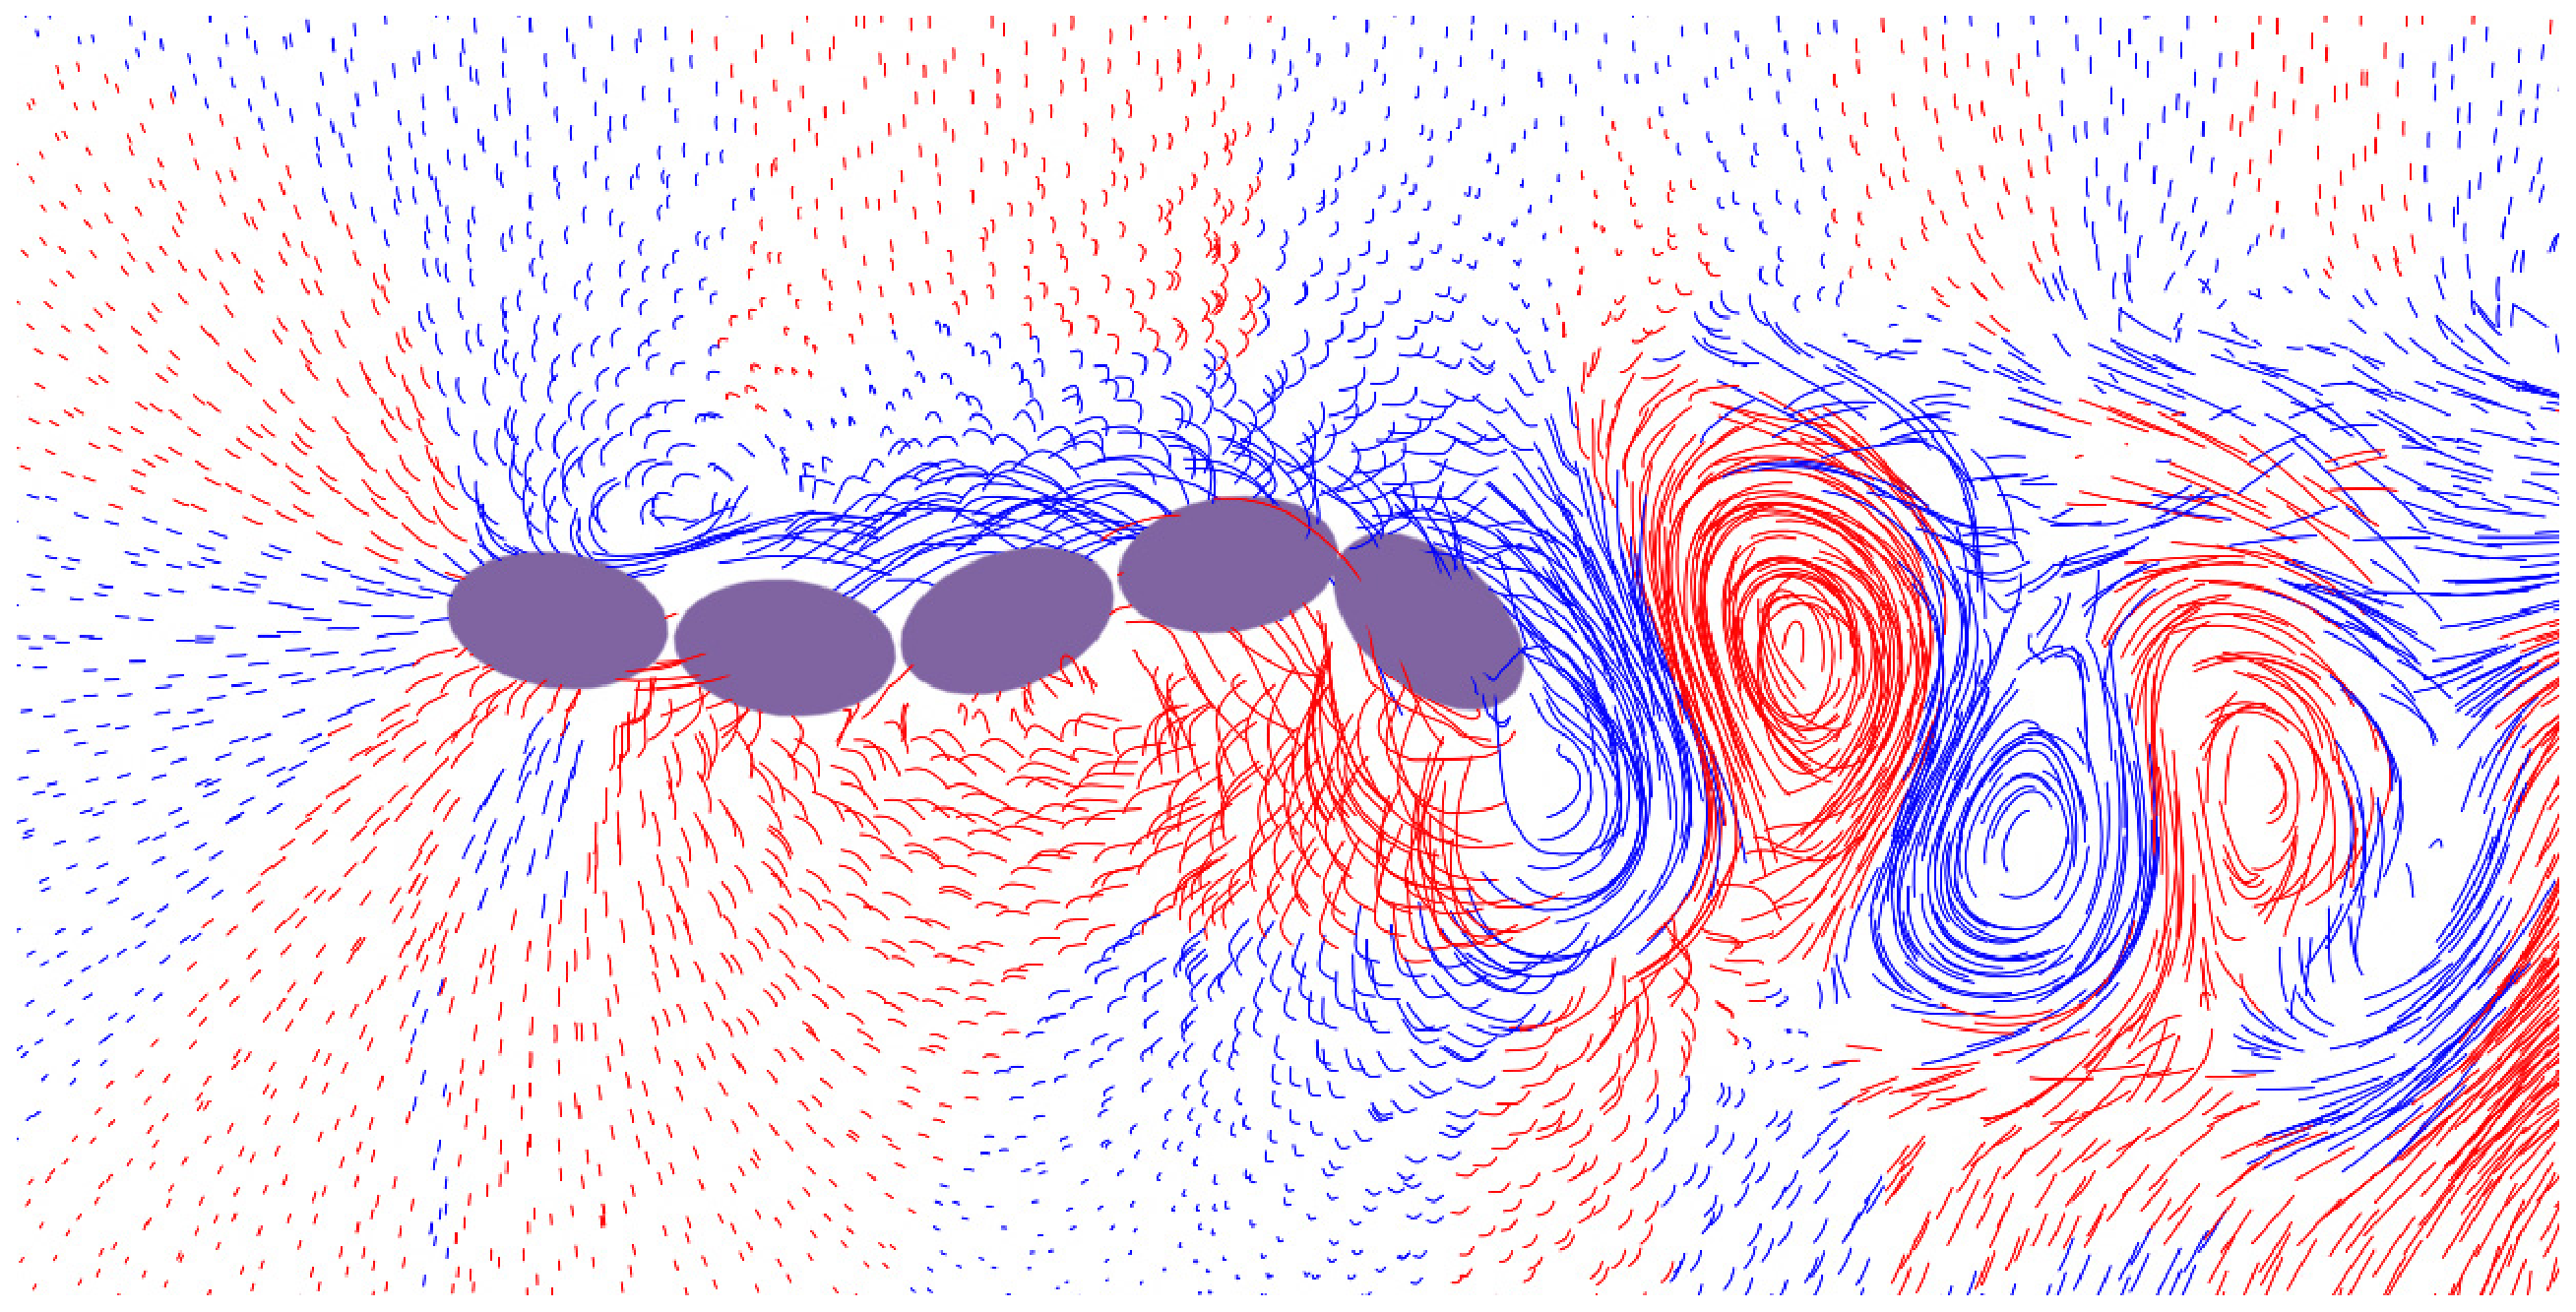
\includegraphics[width=3.2in]{figures/eel2D.eps}
\caption{A five-link eel swims in a 2D fluid environment. In contrast to the simulation in 3D, an eel swimming in 2D fluid sheds only one single vortex street. Red traces show the counter-clockwise vortices while blue traces show the clockwise vortices.}
\label{fig:eel2D}
\end{figure}

Our final example of fish motion is that of a manta ray.  The manta has a
body that is thin in the vertical direction and that has large pectoral fins
that extend in the horizontal direction.  It swims by slow flapping strokes
of these wing-like pectoral fins (the rajiform swimming mode), somewhat like
a slow-motion version of a bird flapping its wings.  Although the manta ray
does not seem to be a good candidate to be modelled as an articulated
figure, we wanted to see how far the articulated models could be pushed.  We
modelled the ray's pectoral fins as four rows of thin plates that are
connected to one another near the leading edge of the fin.  The resulting
swimming motion from the optimization procedure exceeded our expectations,
producing the same graceful flapping that these creatures use to swim (see
Figure~\ref{fig:manta}).

We tested our path following approach using the manta ray model.  We used
our optimization method to find efficient swimming for forward motion, an
upward turn and a downward turn.  We then gave the manta ray a vertical
S-shaped path to follow using our path following controller.  The
simulated ray was able to follow the path quite closely, as the composite
image in Figure~\ref{fig:manta_path} shows.  Note that this path following
motion was created with a single simulation, based on gait switching
between the three learned basic motions. We also tested the path following
algorithm using a simple 2D turtle model. We show that the turtle cannot
swim straight without using the path following technique due to the
accumulation of numerical errors. When the path following technique is
applied, the turtle actively adjusts its swimming motions according to its
position and orientation and successfully swims straight.
\begin{figure*}[t]
\centering

\includegraphics[width=\textwidth]{figures/manta.eps}
\caption{A manta ray swimming forward. Rajiform swimmers swim by slow flapping strokes like a slow-motion version of a bird flapping its wings.}
\label{fig:manta}
\end{figure*}

\begin{figure*}[t]
\centering

\includegraphics[width=\textwidth]{figures/turtle.eps}
\caption{A turtle swims in water with a flapping motion of its two front flippers. }
\label{fig:turtle}
\end{figure*}

\begin{figure}[!b]
\centering

\includegraphics[width=3.2in]{figures/manta_path2.eps}
\caption{A manta ray follows an S-shaped path by choosing maneuvers from ``swimming straight'', ``pitch up'' and ``pitch down''. The red curve is the path specified by the user.}
\label{fig:manta_path}
\end{figure}

\begin{figure*}[ht]
\centering

\includegraphics[width=\textwidth]{figures/frog.eps}
\caption{A frog mainly relies on its large rear legs to provide forward thrust in the water.}
\label{fig:frog}
\end{figure*}


\begin{figure*}[ht]
\centering

\includegraphics[width=\textwidth]{figures/alien.eps}
\caption{An alien aquatic creature that swims in water by undulating its tails and flapping its wings. Note the two pairs of wings are slightly out of phase to mimic flapping motion of larger wings.}
\label{fig:alien}
\end{figure*}




Figure~\ref{fig:turtle} shows the motion of a sea turtle that was created
using optimization.  Adult sea turtles are underwater fliers, moving
themselves forward with a flapping motion of their two front flippers that
is called a \emph{powerstroke}~\cite{wyneken1997}.  Note that our turtle
results show the characteristic rotating of the front flippers during the
upward stroke.  Figure~\ref{fig:frog} shows the results of our swimmer
optimization for a model frog.  As with real frogs, the large rear legs
provide the forward thrust using a classic frog kick. Note that the frog uses its forelimbs with a small range of motion. We think this is because the contribution from the arms is small relative to the contribution from the legs. Based on our observation, some real frogs do not use their forelimbs much when swimming.

In the accompanying video, we also demonstrates that articulated figures
can differ dramatically in their swimming motion depending on whether the
simulated fluid is a simple model or a full Navier-Stokes (NS) solver.
Our simple fluid simulator calculates the force as the square of the
normal component of the velocity of a moving surface element.  This
simplified fluid model is identical to that
in~\cite{Wu:2003,lentine2010creature}.  We show that swimming in
different fluid models leads to different locomotions. Figure~\ref{fig:accordian} shows a 2D swimmer that
compresses and relaxes its body in an accordian-like manner moves through
the water in the NS fluid but stay in one place in the simple fluid. We
demonstrate that the gaits trained in different fluid models differ
considerably.  The swimming gait for a fish trained in NS fluid smoothly
flaps its tail to propel itself forward.  When this same fish model is
optimized using the simple fluid, the resulting motion is considerably
different, gaining thrust mainly from bending at a sharp angle at the
middle joint of the body.  These differences in motion between a simple
fluid and the NS fluid are in agreement with the findings of Lentine et
al.~\cite{lentine2010creature}.

In order to test the generality of our method, we applied our swimming
optimization to an articulated figure that has no counterpart in the real
world (see Figure~\ref{fig:alien}).  This is the swimming version of the task of finding plausible walking
motions for a user-created land
creature~\cite{hecker2008real,wampler2009optimal}.  Our alien creature has two
pairs of limbs on the trunk of its body, and in addition has a long and
powerful tail.  The motion that was found by our optimization combines a
whip-like motion of the tail together with coordinated rowing from the pairs of
limbs.  Although there is no point of comparison in the real world for this
creature's motion, the resulting swimming pattern looks entirely plausible.

\begin{figure}[!b]
\centering
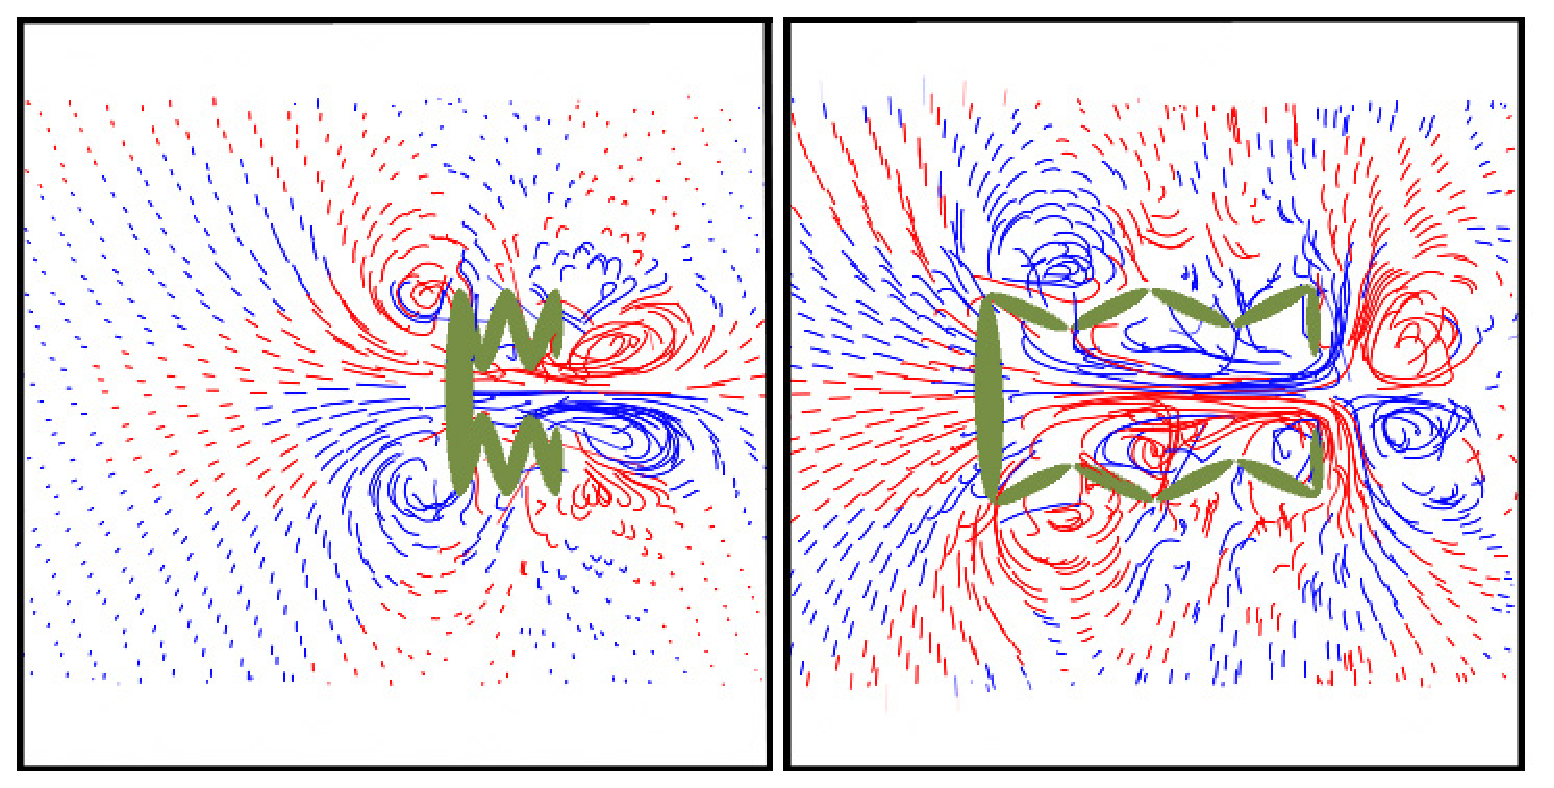
\includegraphics[width=3.2in]{figures/accordian.eps}
\caption{An imaginary creature swims forward by compressing and relaxing its body in an accordion-like manner in a Navier-Stokes fluid model. The images are two snapshots in the animation sequence. This demonstrates that including the Navier-Stokes fluid model is necessary to capture certain swimming patterns, such as jet propulsion, because a simplified fluid model does not allow forward motion for such modes of locomotion.}
\label{fig:accordian}
\end{figure}

Although our method requires little prior knowledge about the swimming gait of the creature,
there are some parameters that users can change, including the energy bound, the period of
the motion for each degree of freedom, and joint limits. This provides users the freedom to
achieve different motion, agile or slow, by changing these parameters. In particular, we tuned the period
of the swimming gait and the energy bound in our examples. We used a period of one second
for all of the examples. We made this choice deliberately because choosing a longer period means longer
optimization time (each CMA sample need to simulate two cycles of swimming motions). However, we believe
that including the period into the optimization will probably give more interesting results because different periods could make
a big difference in the final swimming gait. We leave this as future work. To set the energy bounds, we began by trying out several energy bounds
for an initial animal, the fish shown in the leftmost of Figure~\ref{fig:teaser1}.
Once we were satisfied with the results, we then used this as our standard energy bound.
For a new creature, we scaled this standard energy bound according to the mass of the new creature
relative to the mass of the fish. Users can also change the weights in the objective function.
In our examples, we set all these parameters by intuition without much tuning. The weights
are reported at the end of each paragraph that introduces the different objectives in Chapter \ref{sec:swimmingObj}.

\section{Discussion}

We have demonstrated that our approach creates natural swimming behavior for
a wide variety of animal bodies.  For short-bodied fish and eels, our
results show vortex trails that are in agreement with laboratory
measurements and other published simulation results.  For the other
creatures, our optimized motions have the same overall appearance of the
real-world animals, although lab data is not available.  Our articulated
body representation of creature anatomy is quite general, even allowing us to
animate forms such as the manta ray that are not usually thought of as
articulated figures.

Although we have successfully applied our method to various aquatic
creatures with disparate body shapes and joint configurations, our approach does
have limitations. Our two-way coupling method needs to voxelize the articulated rigid body,
and the accuracy for representing the articulated figure depends on the grid
resolution. Thin features cannot be captured by the fluid simulator (Figure~\ref{fig:grid}). We believe that incorporating adaptive grids
\cite{Losasso04Octree} or unstructured meshes
\cite{Brochu10MatchingElement,klingner2006mesh} can dramatically increase
the accuracy of the two-way coupling. Furthermore, the two-way coupling
method is tailored for the interaction between fluids and articulated
figures. Even though many aquatic creatures have a skeleton and can be
represented well by articulated figures, there are exceptions such as
jellyfish. Our framework for discovering the optimal swimming gaits and
path following is still valid for soft-body creatures, but we would need
an efficient two-way coupling mechanism to simulate these swimming
motions. We leave this as future work.

We use the sine function to parameterize the joint space. There
are quite a few motions that cannot be depicted by a single sine function,
such as gliding. One possible way to improve this is to to use a weighted
sum of multiple sine functions with different amplitudes, phases and
periods \cite{Grzeszczuk95automatedlearning}. However, this would require more
optimization variables and more computational resources to discover a
swimming gait. \newtext{In addition, other simplifications to ease optimization, including enforcing symmetry and hardcoding the swimming frequency to be one hertz, further restrict the motion space to a smaller subset of possible swimming motions employed in nature.}

Our simulated swimmers seem to use more energy than the real creatures do because the simulated water is more viscous than real water. Even though we use the inviscous Navier-Stokes equation (Euler equation) to simulate the fluid, there is numerical viscosity. We chose to use relatively coarse grid, and thus incur large numerical viscosity, to keep the computational time tractable because CMA optimization need to simulate the two-way coupling thousands of times. In addition, while the real aquatic creatures take advantage of their streamline shaped body to reduce the fluid drag, the simulated creatures are voxelized and the resultant stair-step shaped body is not particularly efficient inside the fluid.

There are a number of interesting avenues for future work.  There are many
ways this approach could be expanded to give more control to animators,
including different path following strategies and higher-level behavior
control.  Our work has concentrated on continuous motion, but many animals
have distinctly different movements for situations such as escaping a
predator.  It would be interesting to investigate these faster, intermittent
motions.  Swimming at the \emph{surface} of the water could be studied,
including motions such as a human swimmer doing the crawl or a whale jumping
out of the water (breaching).  Finally, taking a cue from the work of Karl
Sims, it would be fascinating to simultaneously optimize for both swimming
motion and body shape.

\chapter{Ned Land}

Captain Farragut was a good seaman, worthy of the frigate he commanded.
His vessel and he were one.  He was the soul of it.  On the question
of the monster there was no doubt in his mind, and he would not allow
the existence of the animal to be disputed on board.  He believed in it,
as certain good women believe in the leviathan--by faith, not by reason.
The monster did exist, and he had sworn to rid the seas of it.  Either Captain
Farragut would kill the narwhal, or the narwhal would kill the captain.
There was no third course.

The officers on board shared the opinion of their chief.
They were ever chatting, discussing, and calculating the various
chances of a meeting, watching narrowly the vast surface of the ocean.
More than one took up his quarters voluntarily in the cross-trees,
who would have cursed such a berth under any other circumstances.
As long as the sun described its daily course, the rigging was
crowded with sailors, whose feet were burnt to such an extent by
the heat of the deck as to render it unbearable; still the Abraham
Lincoln had not yet breasted the suspected waters of the Pacific.
As to the ship's company, they desired nothing better than to meet
the unicorn, to harpoon it, hoist it on board, and despatch it.
They watched the sea with eager attention.

Besides, Captain Farragut had spoken of a certain sum of two thousand dollars,
set apart for whoever should first sight the monster, were he cabin-boy,
common seaman, or officer.

I leave you to judge how eyes were used on board the Abraham Lincoln.

\section{added section marker}

For my own part I was not behind the others, and, left to no one my share
of daily observations.  The frigate might have been called the Argus,
for a hundred reasons.  Only one amongst us, Conseil, seemed to protest
by his indifference against the question which so interested us all,
and seemed to be out of keeping with the general enthusiasm on board.

\begin{equation}
E=mc^2
\end{equation}

I have said that Captain Farragut had carefully provided his
ship with every apparatus for catching the gigantic cetacean.
No whaler had ever been better armed.  We possessed every
known engine, from the harpoon thrown by the hand to the barbed
arrows of the blunderbuss, and the explosive balls of the duck-gun.
On the forecastle lay the perfection of a breech-loading gun,
very thick at the breech, and very narrow in the bore,
the model of which had been in the Exhibition of 1867.
This precious weapon of American origin could throw with ease
a conical projectile of nine pounds to a mean distance
of ten miles.

Thus the Abraham Lincoln wanted for no means of destruction; and, what was
better still she had on board Ned Land, the prince of harpooners.

Ned Land was a Canadian, with an uncommon quickness of hand, and who knew
no equal in his dangerous occupation.  Skill, coolness, audacity, and cunning
he possessed in a superior degree, and it must be a cunning whale to escape
the stroke of his harpoon.

Ned Land was about forty years of age; he was a tall man
(more than six feet high), strongly built, grave and taciturn,
occasionally violent, and very passionate when contradicted.
His person attracted attention, but above all the boldness
of his look, which gave a singular expression to his face.

Who calls himself Canadian calls himself French; and, little communicative
as Ned Land was, I must admit that he took a certain liking for me.
My nationality drew him to me, no doubt.  It was an opportunity for him
to talk, and for me to hear, that old language of Rabelais, which is still
in use in some Canadian provinces.  The harpooner's family was originally
from Quebec, and was already a tribe of hardy fishermen when this town
belonged to France.

Little by little, Ned Land acquired a taste for chatting, and I
loved to hear the recital of his adventures in the polar seas.
He related his fishing, and his combats, with natural poetry
of expression; his recital took the form of an epic poem,
and I seemed to be listening to a Canadian Homer singing the Iliad
of the regions of the North.

\begin{equation}
E=mc^2
\end{equation}

I am portraying this hardy companion as I really knew him.
We are old friends now, united in that unchangeable friendship
which is born and cemented amidst extreme dangers.  Ah, brave Ned!
I ask no more than to live a hundred years longer, that I may have more
time to dwell the longer on your memory.

Now, what was Ned Land's opinion upon the question of the marine monster?
I must admit that he did not believe in the unicorn, and was
the only one on board who did not share that universal conviction.
He even avoided the subject, which I one day thought it my duty
to press upon him.  One magnificent evening, the 30th July (that is
to say, three weeks after our departure), the frigate was abreast
of Cape Blanc, thirty miles to leeward of the coast of Patagonia.
We had crossed the tropic of Capricorn, and the Straits of Magellan
opened less than seven hundred miles to the south.  Before eight
days were over the Abraham Lincoln would be ploughing the waters
of the Pacific.

Seated on the poop, Ned Land and I were chatting of one thing
and another as we looked at this mysterious sea, whose great
depths had up to this time been inaccessible to the eye of man.
I naturally led up the conversation to the giant unicorn, and examined
the various chances of success or failure of the expedition.
But, seeing that Ned Land let me speak without saying too much himself,
I pressed him more closely.

``Well, Ned,'' said I, ``is it possible that you are not convinced
of the existence of this cetacean that we are following?
Have you any particular reason for being so incredulous?''

The harpooner looked at me fixedly for some moments
before answering, struck his broad forehead with his hand
(a habit of his), as if to collect himself, and said at last,
``Perhaps I have, Mr. Aronnax.''

``But, Ned, you, a whaler by profession, familiarised with all
the great marine mammalia---YOU ought to be the last to doubt
under such circumstances!''

``That is just what deceives you, Professor,'' replied Ned.
``As a whaler I have followed many a cetacean, harpooned a great number,
and killed several; but, however strong or well-armed they may
have been, neither their tails nor their weapons would have been
able even to scratch the iron plates of a steamer.''

``But, Ned, they tell of ships which the teeth of the narwhal
have pierced through and through.''

``Wooden ships---that is possible,'' replied the Canadian,
``but I have never seen it done; and, until further proof,
I deny that whales, cetaceans, or sea-unicorns could ever produce
the effect you describe.''

``Well, Ned, I repeat it with a conviction resting on the logic of facts.
I believe in the existence of a mammal power fully organised, belonging to
the branch of vertebrata, like the whales, the cachalots, or the dolphins,
and furnished with a horn of defence of great penetrating power.''

``Hum!'' said the harpooner, shaking his head with the air of a man
who would not be convinced.

``Notice one thing, my worthy Canadian,'' I resumed.
``If such an animal is in existence, if it inhabits the depths
of the ocean, if it frequents the strata lying miles below
the surface of the water, it must necessarily possess an
organisation the strength of which would defy all comparison.''

``And why this powerful organisation?'' demanded Ned.

``Because it requires incalculable strength to keep one's self
in these strata and resist their pressure.  Listen to me.
Let us admit that the pressure of the atmosphere is represented
by the weight of a column of water thirty-two feet high.
In reality the column of water would be shorter, as we are
speaking of sea water, the density of which is greater than
that of fresh water.  Very well, when you dive, Ned, as many
times 32 feet of water as there are above you, so many times
does your body bear a pressure equal to that of the atmosphere,
that is to say, 15 lb.  for each square inch of its surface.
It follows, then, that at 320 feet this pressure equals
that of 10 atmospheres, of 100 atmospheres at 3,200 feet,
and of 1,000 atmospheres at 32,000 feet, that is, about 6 miles;
which is equivalent to saying that if you could attain this
depth in the ocean, each square three-eighths of an inch
of the surface of your body would bear a pressure of 5,600 lb.
Ah! my brave Ned, do you know how many square inches you carry on
the surface of your body?''

``I have no idea, Mr. Aronnax.''

``About 6,500; and as in reality the atmospheric pressure is about 15 lb.
to the square inch, your 6,500 square inches bear at this moment a pressure
of 97,500 lb.''

``Without my perceiving it?''

''Without your perceiving it.  And if you are not crushed by
such a pressure, it is because the air penetrates the interior
of your body with equal pressure.  Hence perfect equilibrium
between the interior and exterior pressure, which thus neutralise
each other, and which allows you to bear it without inconvenience.
But in the water it is another thing.''

``Yes, I understand,'' replied Ned, becoming more attentive;
``because the water surrounds me, but does not penetrate.''

``Precisely, Ned:  so that at 32 feet beneath the surface of the sea you would
undergo a pressure of 97,500 lb.; at 320 feet, ten times that pressure;
at 3,200 feet, a hundred times that pressure; lastly, at 32,000 feet,
a thousand times that pressure would be 97,500,000 lb.---that is to say,
that you would be flattened as if you had been drawn from the plates of
a hydraulic machine!''

``The devil!'' exclaimed Ned.

``Very well, my worthy harpooner, if some vertebrate, several hundred
yards long, and large in proportion, can maintain itself in such depths---of
those whose surface is represented by millions of square inches, that is
by tens of millions of pounds, we must estimate the pressure they undergo.
Consider, then, what must be the resistance of their bony structure,
and the strength of their organisation to withstand such pressure!''

``Why!'' exclaimed Ned Land, ``they must be made of iron plates
eight inches thick, like the armoured frigates.''

``As you say, Ned.  And think what destruction such a mass would cause,
if hurled with the speed of an express train against the hull of a vessel.''

``Yes---certainly---perhaps,'' replied the Canadian, shaken by these figures,
but not yet willing to give in.

``Well, have I convinced you?''

``You have convinced me of one thing, sir, which is that,
if such animals do exist at the bottom of the seas, they must
necessarily be as strong as you say.''

``But if they do not exist, mine obstinate harpooner, how explain
the accident to the Scotia?''

\chapter{Locomotion with a Passive Mechanical Device}
\section{Motivation}

The invention of tools has greatly increased the efficiency of our work and the quality of our lives. The bicycle is such an invention that has drastically improved the efficiency of human locomotion. In fact, it was voted as the best invention since the 19th century \cite{BBC2005} because it is an inexpensive, fast, healthy and environmentally friendly mode of transportation. However, riding a bicycle is nontrivial due to its inherently unstable dynamics: The bike will fall without forward momentum and the appropriate human control. Getting onto the bike, balancing, steering and riding on bumpy roads all impose different challenges to the rider. As one important child development milestone, learning to ride a bicycle often requires weeks of practice. We are interested to find whether it is possible to use a computer to mirror this learning process. In addition to the basic maneuvers, the most skillful riders can jump over obstacles, lift one wheel and balance on the other, and perform a large variety of risky but spectacular bicycle stunts. Performing stunts requires fast reaction, precise control, years of experience and most importantly, courage, which challenges most people. Can we design an algorithm that allows computers to automatically learn these challenging but visually exciting bicycle stunts?

Designing an algorithm to learn to ride a bicycle presents unique challenges. Riding a bicycle involves complex interactions between a human rider and a bicycle. While the rider can actively control each joint, the bicycle is a passive system that can only be controlled by the human rider. To control a single degree of freedom (DOF) of a bicycle, coordinated motions of multiple DOFs of the rider are required. Moreover, the main difficulty in locomotion is to control an under-actuated system by exploiting external contact forces. Manipulating contact forces on a bicycle is indirect. All of the rider's control forces need to first go through the bicycle dynamics to affect the ground reaction forces and vice versa. This extra layer of bicycle dynamics between the human control and the contact forces adds another layer of complexity to the locomotion control. Balance on a bicycle is challenging and it is different from balance when standing or walking. While a human can stand stably due to the large contact area of the feet, a static bicycle cannot stay upright due to its narrow tires. Humans can balance during walking by planning and changing their foot placement. In contrast, the bike rider cannot abruptly change the contact position, which can only be changed gradually through steering. The limited range of human motion on a bicycle makes balance even harder. When the character's hands are constrained to hold the handlebar and their feet are on the pedals, the character loses much of the freedom to move various body parts. He or she cannot employ ankle or hip postural strategies or wave their arms to effectively regulate the linear and the angular momenta.

Balance during bicycle stunts is far more challenging than normal riding. As a stunt example that illustrates the balance issues we plan to tackle, consider a bicycle endo (the third image of Figure~\ref{fig:teaser3}), in which the rider lifts the rear wheel of the bicycle and keeps balance on the front wheel. In this pose, the rider encounters both the longitudinal and lateral instabilities. The small contact region of one wheel and the lifted center of mass (COM) due to the forward leaning configuration exacerbate the balance problem. Furthermore, the off-the-ground driving wheel makes any balance strategies that involve acceleration impossible. The unstable configurations and the restricted actions significantly increase the difficulty of balance during a stunt.

This chapter describes a complete system for controlling a human character that is riding a bicycle in a physically simulated environment. The system consists of two main components: simulating the motion and optimizing the control policy. We simulate the bicycle and the rider as an articulated rigid body system, which is augmented with specialized constraints for bicycle dynamics. The second component provides an automatic way to learn control policies for a wide range of bicycle maneuvers. In contrast to many optimal control algorithms that leverage the dynamics equations to compute the control signals, we made a deliberate choice not to exploit the dynamics equations in our design of the control algorithm. We believe that learning to ride a bicycle involves little reasoning about physics for most people. A four-year-old can ride a bicycle without understanding any physical equations. Physiological studies show that learning to ride a bicycle is a typical example of implicit motor learning \cite{Chambaron2009}, in which procedural memory guides our performance without the need for conscious attention. Procedural memory is formed and consolidated through repetitive practice and continuous evolution of neural processes. Inspired by the human learning process, we formulate a partially observable Markov decision process (POMDP) and use policy search to learn a direct mapping from perception to reaction (procedural memory).

Both prior knowledge of bicycle stunts and an effective searching algorithm are essential to the success of policy search. After studying a variety of stunts, we classify them into two types. We apply feed-forward controllers for the \emph{momentum-driven} motions and feedback controllers for the \emph{balance-driven} ones. We study videos of stunt experts to understand their reactions under different situations and used this information to design the \emph{states} and the \emph{actions} of our controllers. We employ a neural network evolution method to simultaneously optimize both the parametrization and the parameters of the feedback controllers. The way we incorporate the prior knowledge into our system and the effective evolutionary method are both essential to the success of policy search.

We evaluate our system by demonstrating a human character riding different types of bicycles and performing a wide variety of stunts (Figure \ref{fig:teaser3}). We also evaluate the importance of optimizing the parametrization of a policy. We share our experiences with different reinforcement learning algorithms that we have tried throughout this research project.


\section{Overview}
\begin{figure}[!t]
  \centering
  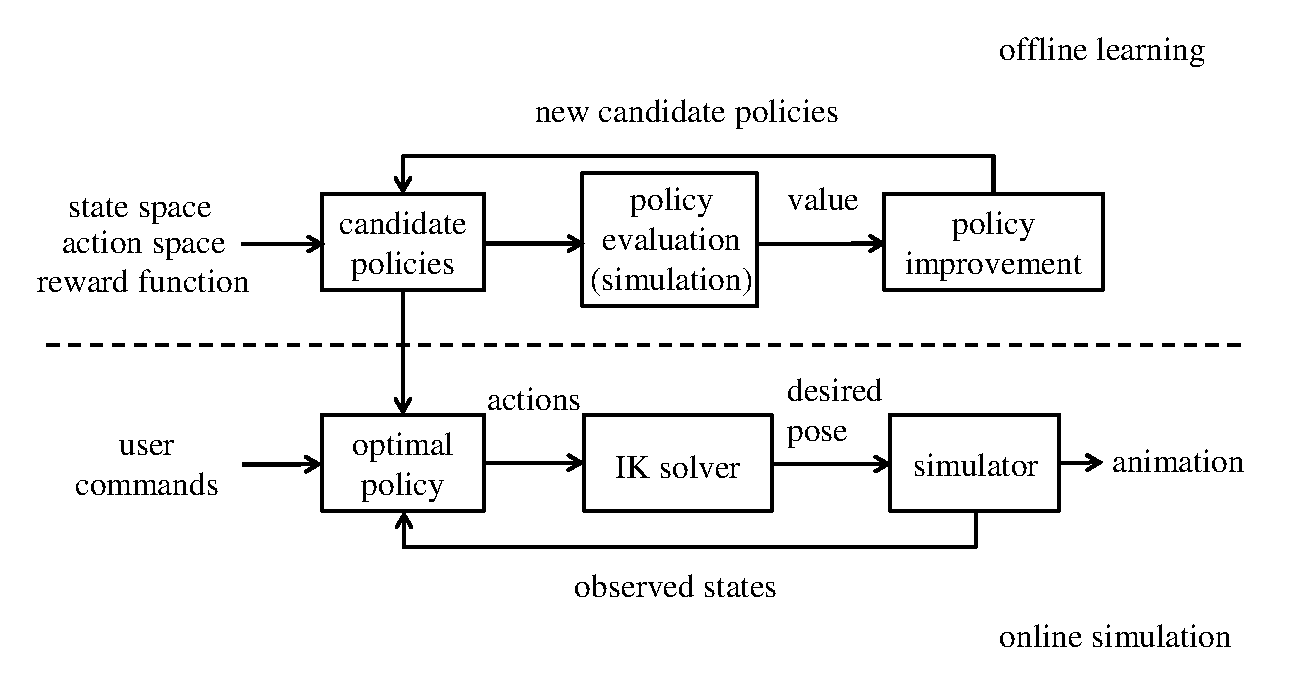
\includegraphics[width=5.5in]{figures/overview}
  \caption{Overview of our algorithm.}
  \label{fig:overview}
\end{figure}

We have designed a system that allows a virtual human character to learn to ride a bicycle and perform a wide variety of stunts. The goal of our system is to learn a control policy that initiates a particular action at any state. Given the state space, the action space and the reward function for each bicycle task, the offline learning subsystem starts with an initial set of candidate policies, iteratively evaluates (using simulation) and evolves them (using CMA or NEAT) until the optimal policy is found. This optimal policy allows the user to interact with the bicycle simulation in real time by giving commands such as steering to the left. The online simulation subsystem first extracts the observable states, such as the tilt angle, the falling speed, and the actual and the user-specified handlebar angle. It then queries the policy to determine appropriate actions, such as turning the handlebar at a certain speed to fulfill the user's command while still maintain the balance of the bicycle. Executing actions, such as turning the handlebar, requires a coordinated full-body motion of the rider. An Inverse Kinematics (IK) solver maps the compact set of actions to the rider's full-body pose. The simulator tracks this desired pose and at the same time simulates the dynamics of both the human rider and the bicycle. Figure \ref{fig:overview} illustrates the main components of our system.

\section{Bicycle and Rider Simulation}
Our simulator is based on Open Dynamic Engine (ODE) \cite{ode:2008},
but we augmented it with additional constraints to simulate both the
bicycle and the human rider. We treat the bicycle and the rider as a
system of articulated rigid bodies. Since the dynamics is represented
in the maximal coordinates, each rigid body has six DOFs and its
dynamic equation is
\begin{equation}
\left[\begin{array}{cc}
\vc{M} & \vc{0} \\
\vc{0} & \vc{I}
\end{array}\right]
\left[\begin{array}{c}
\dot{\vc{v}} \\
\dot{\vc{\omega}}
\end{array}\right]=
\left[\begin{array}{c}
m\vc{g} \\
-\dot{\vc{I}}\vc{\omega}
\end{array}\right]
+\vc{J}^T
\left[\begin{array}{c}
\vc{f}\\
\vc{\tau}
\end{array}\right]
\label{eq:dynamics}
\end{equation}
where $\vc{M}$ is the mass matrix, $\vc{I}$ is the inertia tensor, $\vc{v}$ and $\vc{\omega}$ are the linear and angular velocities, $\vc{f}$ and $\vc{\tau}$ are the constraint forces and torques, which come from the bicycle chains, the joints, the actuators and the contacts. $\vc{J}^T$ is the transposed Jacobian matrix that maps the constraint forces and torques to the body.

Chains transfer power from the pedals to the rear wheel on a bicycle. We use a linear equality constraint to realize the effect of a bicycle chain.
\begin{equation}
\vc{n}^T(\alpha\vc{\omega}_A-\vc{\omega}_B)=0
\label{eq:chainConstraint}
\end{equation}
where bodies $A$ and $B$ are the pedals and the rear wheel. $\vc{n}$ is the common direction of their rotational axes and $\alpha$ represents the gear ratio, which is the ratio between the number of teeth on the chain-ring and the number on the rear sprocket. Note that eq.~(\ref{eq:chainConstraint}) models a fixed-gear bicycle. In some tasks, we disabled this constraint to mimic the effect of the free wheel, allowing the rider to glide without pedaling.

The other constraints are standard from the implementation of ODE. For completeness of presentation, we include a brief description of such constraints in Appendix \ref{chapter:AppendixB}. Note that we use the actuator constraints instead of the traditional PD servos to track a desired pose. We have found that using the actuator constraints enables us to simulate at large time steps (0.01s), which significantly speeds up the computation.

We made several simplifications in the simulation. We used ball joints to attach the rider's feet to the pedals. This treatment is similar to wearing toe clips in the real world. We also used ball joints to connect the rider's hands with the handlebar. For some tasks in which the rider is seated, we further constrained the relative position and orientation between the rider's pelvis and the bicycle seat.


\section{Learning to Ride a Bicycle}
\label{sec:control}

\subsection{Markov Decision Process}
We formulate the bicycle control problem as a POMDP. A Markov decision process (MDP) is a tuple $(S, A, R, D, P_{sas'}, \gamma)$, where $S$ is the \emph{state} space; $A$ is the \emph{action} space; $R$ is the \emph{reward function}; $D$ is the distribution of the initial state $s_0$; $P_{sas'}$ is the transition probability; and $\gamma \in [0, 1]$ is the discount factor. For example, in the bicycle balance task, we choose the state space $S$ to include the tilt angle of the bike, the tilting speed and the handlebar angle. We choose the action $A$ to be turning the handlebar at a certain speed. We choose the reward function $R$ at the state $s$ to be
\begin{equation}
\begin{array}{ll}
R(s) = & \left\{ \begin{array}{ll}
1 & \textrm{if the bicycle remains upright,}\\
0 & \textrm{otherwise.}
\end{array} \right. \\
\end{array}
\label{eq:balanceReward}
\end{equation}
The initial state $s_0$ is drawn from a random perturbation near the upright orientation of the bicycle. The state transition is calculated using simulation, and we do not discount the rewards ($\gamma = 1$).

A \emph{policy} is a mapping from states to actions: $\pi : S \mapsto A$. The \emph{return} of a policy is the accumulated rewards along the state trajectory starting at $s_0$ by following the policy $\pi$ for $N$ steps.
\begin{displaymath}
V^\pi(s_0)=\sum_{i=0}^N{R(s_i)}
\end{displaymath}
The \emph{value} of a policy is the expected return with respect to the random initial state $s_0$ drawn from D.
\begin{equation}
V(\pi)=E_{s_0\sim D}[V^\pi(s_0)]
\label{eq:policyValue}
\end{equation}
The optimal solution of an MDP is the policy that has the maximum value $\pi^*=\arg\max_\pi V(\pi)$. The optimal policy in the bicycle balance example decides how to turn the handlebar under different situations so that the bicycle can stay upright for the longest time.

Our MDP is partially observable because we choose to observe only a selected subset of all the simulation states. We have found that focusing on a small number of relevant states for each task results in a more efficient learning process. The actions are also selected based on our prior knowledge of the task. Table~\ref{table:states} and~\ref{table:actions} summarize all the states and actions used across our different examples. The 25 states in Table~\ref{table:states} may seem exhaustive, but we only use a subset of them (typically not more than eight states) for each task.

\begin{table}[!t]
\centering
\begin{tabular}{|l|l|}
\hline
state & description \\
\hline
$t$    & time (used in the feed-forward controllers)\\
$\theta$ & handlebar angle \\
$\alpha$    & roll angle of the bike (tilt left/right)   \\
$\dot{\alpha}$     & roll speed  \\
$\beta$     & pitch angle of the bike  \\
$\dot{\beta}$     & pitch speed  \\
$\gamma$     & yaw angle of the bike \\
$\dot{\gamma}$ & yaw speed \\
$v_r$ & rear wheel linear speed \\
$v_f$    & front wheel linear speed  \\
$h_r$     & rear tire height above the ground  \\
$h_f$     & front tire height above the ground  \\
$x$    & pelvis position along x-axis\\
$y$    & pelvis position along y-axis\\
$z$    & pelvis position along z-axis\\
$\phi$    & torso orientation in the Sagittal plane\\
$\psi$    & torso orientation in the Coronal plane\\
$\chi$   & torso orientation in the Transverse plane\\
$\dot{\phi}$    & torso angular speed in the Sagittal plane\\
$\dot{\psi}$    & torso angular speed in the Coronal plane \\
$\dot{\chi}$   & torso angular speed in the Transverse plane\\
$\Delta\theta $ & difference between actual and desired handlebar angle \\
$\Delta\beta$    & difference between actual and desired pitch angle\\
$\Delta v_r $ & difference between actual and desired rear wheel speed \\
$\Delta v_f $ & difference between actual and desired front wheel speed \\
\hline
 \end{tabular}
 \caption{States and their descriptions. The rider's pelvis position, torso orientation and angular velocity are calculated in the bicycle frame's coordinates.}
 \label{table:states}
 \end{table}

\begin{table}[!t]
  \centering
\begin{tabular}{|l|l|}
\hline
action & description \\
\hline
$\dot{\theta}$ & steering\\
$\dot{v}_r $ & accelerating or braking\\
$\dot{v}_f $ & accelerating or braking on a front-wheel-driven bicycle\\
$\tau_f$    & front braking   \\
$\dot{x}$     & pelvis motion along x-axis\\
$\dot{y}$     & pelvis motion along y-axis\\
$\dot{z}$     & pelvis motion along z-axis\\
$\dot{\phi}$    & torso motion in the Sagittal plane\\
$\dot{\psi}$    & torso motion in the Coronal plane \\
$\dot{\chi}$   & torso motion in the Transverse plane\\
$\tilde{x}$     & desired pelvis position along x-axis\\
$\tilde{y}$     & desired pelvis position along y-axis\\
$\tilde{z}$     & desired pelvis position along z-axis\\
$\tilde{\phi}$    & desired torso orientation in the Sagittal plane\\
\hline
\end{tabular}
\caption{Actions and their descriptions. The rider's pelvis and torso movements are relative to the bicycle frame's coordinates.}
\label{table:actions}
\end{table}


\subsection{Policy Search}
We apply policy search to optimize the control policies. Unlike value iteration, policy search can be easily applied to MDPs in high dimension and with continuous state and action spaces. This algorithm searches for the optimal policy within a parameterized functional space $\pi^*\in\Pi$. During policy search, one or more random policies are generated as an initial guess. These candidates are evaluated and improved iteratively. Policy improvement can be guided using the policy gradient \cite{Ng:2000:PPS}, trajectory optimization \cite{Levine2013} or other optimization techniques \cite{Heidrich-Meisner:2008}. Policy search ends when the iteration converges or the maximum number of iterations is reached.


\subsubsection{Policy Parametrization}
\label{sec:parametrization}

\begin{figure}[!t]
  \centering
  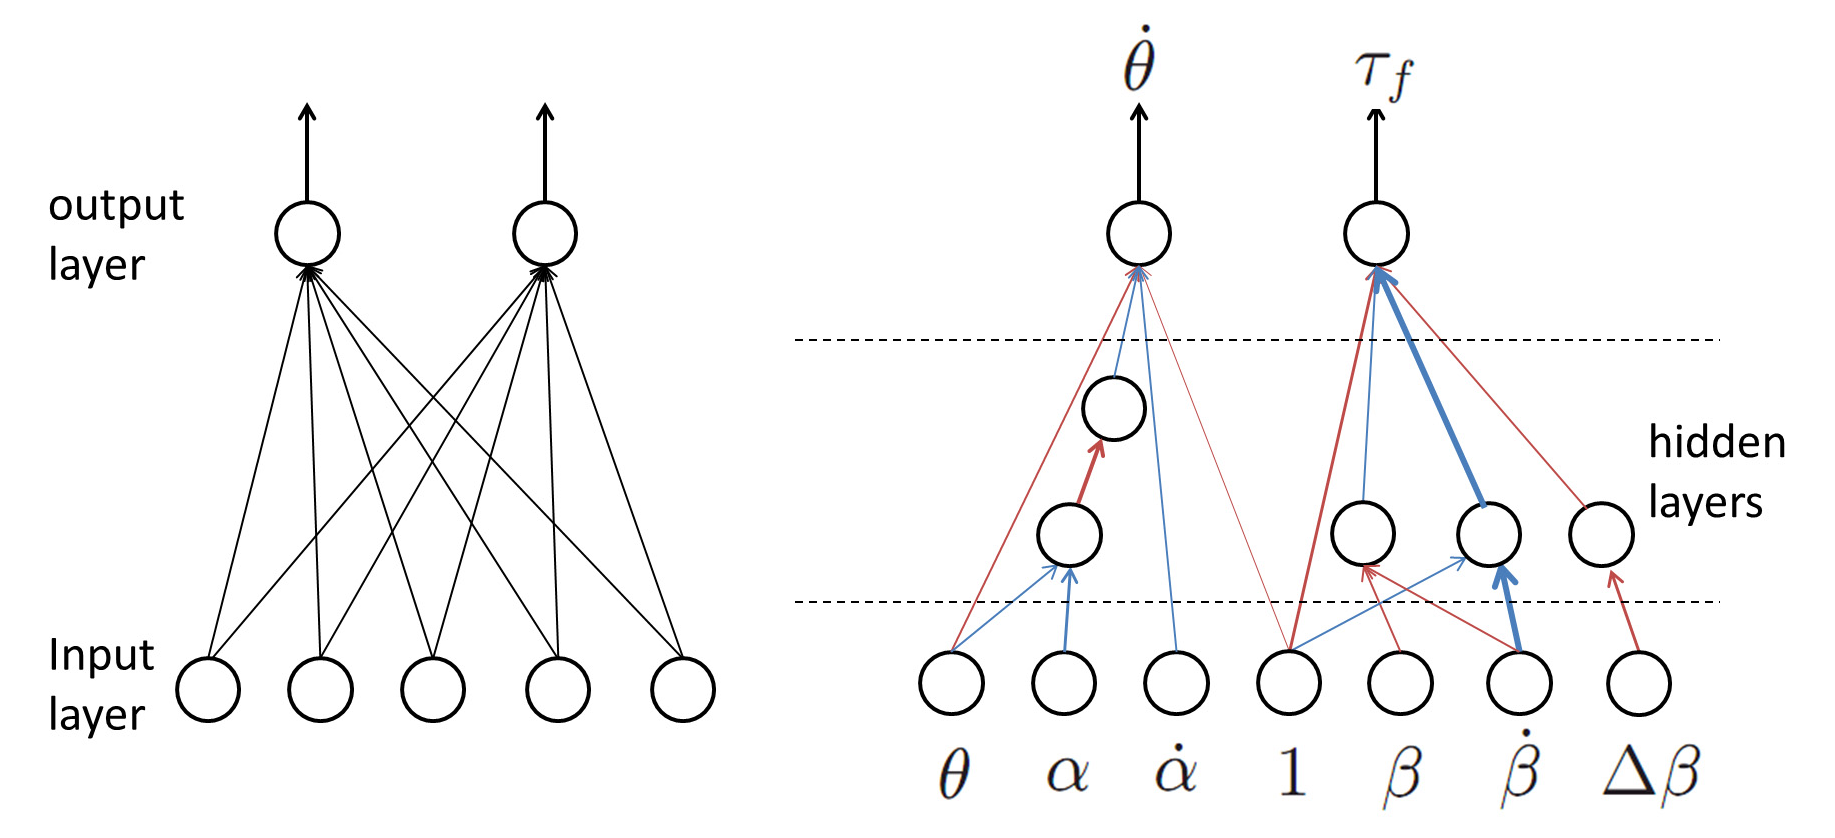
\includegraphics[width=3.4in]{figures/simpleNetwork}
  \caption{Left: A simple neural network with input and output layers that are directly connected. Right: A neural network learned using our algorithm for balancing on the front wheel. Blue arrows mean negative weights while red mean positive weights. The width of the arrows encodes the magnitude of the weights. }
  \label{fig:simpleNetwork}
\end{figure}

We use two types of parametrizations for the bicycle control problem: splines for feed-forward control and neural networks for feedback control. We found that most of the stunts can be categorized into momentum-driven, balance-driven or a combination of the two. The momentum-driven stunts involve vigorous full body motions to manipulate the bicycle to a desired orientation. Coordinated full body motions with large magnitude are essential, but the short duration of this type of stunts makes balance easy to maintain. For this reason, we use feed-forward controllers and represent the action trajectories as cubic Hermite splines. Assuming that the number of control points is given, the parameters to optimize are the time and the value of the control points\footnote{We do not optimize the tangents at the control points and we set them to be zero.}.

Balance-driven stunts require that the rider carefully adjusts his or her COM and maintains a stunt pose for a longer period of time. Feedback balance control is vital to the duration of the performance, which determines the success or failure of the stunt. We use neural networks for their ability to approximate a wide range of functions. The inputs to a network are the observed states, and the outputs are the actions. Figure~\ref{fig:simpleNetwork} Left illustrates a simple neural network that directly connects the input and the output layers. The output of neuron $i$ is
\begin{displaymath}
v_i=\sigma(\sum_j w_{ij} v_j)
\end{displaymath}
where $w_{ij}$ is the connection weight between neuron $i$ and $j$, and $\sigma$ is the sigmoid function $\sigma(x) = 1/(1+e^{-x})$.

Parametrization determines the potential quality of the optimal policy. The network shown in Figure~\ref{fig:simpleNetwork} Left is too simple for representing a complex policy required by bicycle stunts. However, it is not clear how to manually design the network structure, given the control policies of unsuccessful stunts. For this reason, we use NEAT to search for both the structure of the neural network and its weights simultaneously, which finds far better policies than searching over a fixed network. Figure~\ref{fig:simpleNetwork} Right demonstrates the learned network for the balance task of a bicycle endo using NEAT. See Chapter~\ref{sec:improvement} for more details.

\subsubsection{Policy Evaluation}
To evaluate a policy, we formulate a reward function in the following form:
\begin{equation}
R(s)=R_t(s)+wR_r(s)
\end{equation}
where $R_t$ and $R_r$ are task-specific and regularization terms respectively. $w$ is the weight.

We use eq.(\ref{eq:balanceReward}) as the task-specific reward for balance-driven tasks. As the reward is accumulated over time, the return counts the number of frames that the bicycle stays upright. The task-specific reward varies for each momentum-driven stunt. For example, the reward for initiating an endo (lifting the rear wheel) is to maximize the negative pitch angle of the bike $R_t=-\beta$. We refer the readers to Chapter \ref{sec:results} and for more detailed descriptions of task-specific rewards.

Given the task-specific reward term alone, multiple optimal policies could exist. Taking the balance task as an example, a policy that rides in a straight line and another that oscillates in a sinusoidal path by periodically swinging the handlebar can both balance well and thus yield the same value. The regularization term is mainly used to eliminate this ambiguity. We use the regularization term $R_r=\frac{1}{|\theta|+\epsilon}$ to express our preference of riding straight. In our examples, all the regularizers are in the form of
\begin{displaymath}
R_r = \frac{1}{|X|+\epsilon}
\end{displaymath}
where $X$ can be substituted by $\alpha$ for the upright bicycle position, $\Delta \theta$ for the desired steering angle, $\Delta \beta$ for the desired pitch angle, $\Delta v$ for the desired speed, $(x, y, z)$ and $(\phi, \psi, \chi)$ for small changes of rider's pelvis position and torso orientation. A small number $\epsilon$ in the denominator is used to bound the reward.

We do not explicitly minimize the rider's effort in the reward function because it is difficult to balance the effort minimization objective and the task-specific objective for difficult stunt actions. However, we limit the maximum actuated joint torques of the rider in the simulation to ensure that the rider does not possess super-human strength.

We run multiple simulations with different initial configurations $s_0$, which are sampled from random perturbations of the default bicycle velocity and orientation, to evaluate the value of a policy. At each simulation step, our algorithm calculates the reward for the current state, and accumulates this until the bicycle falls or after 1000 time steps. The average return of all the simulations is the value of the policy.

\subsubsection{Policy Improvement}
\label{sec:improvement}

Many policy improvement methods utilize the policy gradient \cite{Peters:2008} to perform iterative ascending operations. However, our simulation of bicycle stunts involves frequent discrete events such as establishing and breaking contact, which invalidates the gradient information. For this reason, we use sample-based stochastic optimization techniques. We apply CMA to search for the feed-forward controllers since the parametrization of splines is fixed. We use NEAT to search for feedback controllers, including the structure and the weights of the neural network. NEAT has many similarities to genetic algorithms, but it is tailored to the creation of neural networks. We will describe NEAT briefly below. For further details we refer readers to the original paper \cite{Stanley:2002:ENN}.

NEAT iteratively performs evaluation, selection, crossover and mutation. To maximize the value of a policy, NEAT starts with a simple network structure, in which the input and the output layers are directly connected. A population of such networks with random weights is drawn as an initial guess. These candidate policies are evaluated and the top 20\% are selected to survive. Pairs of randomly-selected surviving policies are crossed over to produce a new generation (more on this below). Mutations (with low probability) can perturb connection weights, add a neuron or add a connection. Note that the addition of a neuron or a connection complexifies the network structure and enriches the class of functions that it can represent.

Crossover is nontrivial in NEAT because the parent neural networks can have different topologies. To overcome this difficulty, the newly-added neuron or connection is assigned a unique innovation number, which tells the history of the mutation and how to match up neurons or connections between parents during crossover. The neurons or connections that share the same innovation number across parents are from the same ancestor, which will be inherited randomly by the child sample. The neurons or connections that have no counterparts in the other parent are from different mutations. They will be inherited from the parent with the higher value.

The evolution ends when the policy values do not increase over a certain number of iterations or the maximum number of iterations is reached.

\section{Results}
\label{sec:results}

In this section we describe the results of our system. Please watch the video\footnote{https://dl.dropboxusercontent.com/u/36899427/siggraph2014.mp4} for the bicycle riding and stunt
animations. Our system was implemented in C++, and we used ODE with additional chain constraints to simulate both the bicycle and the human rider. The simulator runs in real time on a desktop workstation with a 2.26GHz CPU and 4GB of memory. We generated 90 samples per iteration and 50 iterations for offline policy search. The computations were distributed across 16 CPU cores on a cluster. The learning time ranges from a few minutes to half an hour depending on the number of simulations used to estimate the expected return (eq.~\ref{eq:policyValue}). Table~\ref{table:stateActions} summarizes the choices of states and actions for each bicycle task.

We designed three different bicycles and a unicycle to test our controllers on a variety of tasks. \emph{Road bikes} (Figure~\ref{fig:balance}) are designed to travel at speed on paved roads. They have very narrow tires to reduce the rolling resistance. The seats are mounted high so that the riders can bend their upper bodies down for less air resistance. We use a \emph{BMX bike} (Figure~\ref{fig:endo}) for stunts. BMX bikes are usually considerably smaller for nimble and agile handling. They have fat tires to facilitate balance and to increase traction. BMX bicycle parts can often be customized to meet the needs of different stunts. \emph{High wheelers} (Figure~\ref{fig:highwheeler}) are an old style of bicycle appearing in the late 19th century. They have a large front wheel and a much smaller rear wheel. This peculiar design makes high wheelers difficult to ride due to the center of mass being high and not far behind the front wheel. Any sudden stop could send the rider over the handlebars. A \emph{unicycle} (Figure~\ref{fig:unicycle}) has only one wheel and no handlebar. The rider needs to be concerned about the balance in both the longitudinal and the lateral directions. Different cycle designs greatly affect the handling characteristics and change the behavior of the riders. This variety puts the generality of our algorithm to the test. We modeled all the cycles and calculated their mass properties in SolidWorks.

\begin{figure*}[!t]
\centering
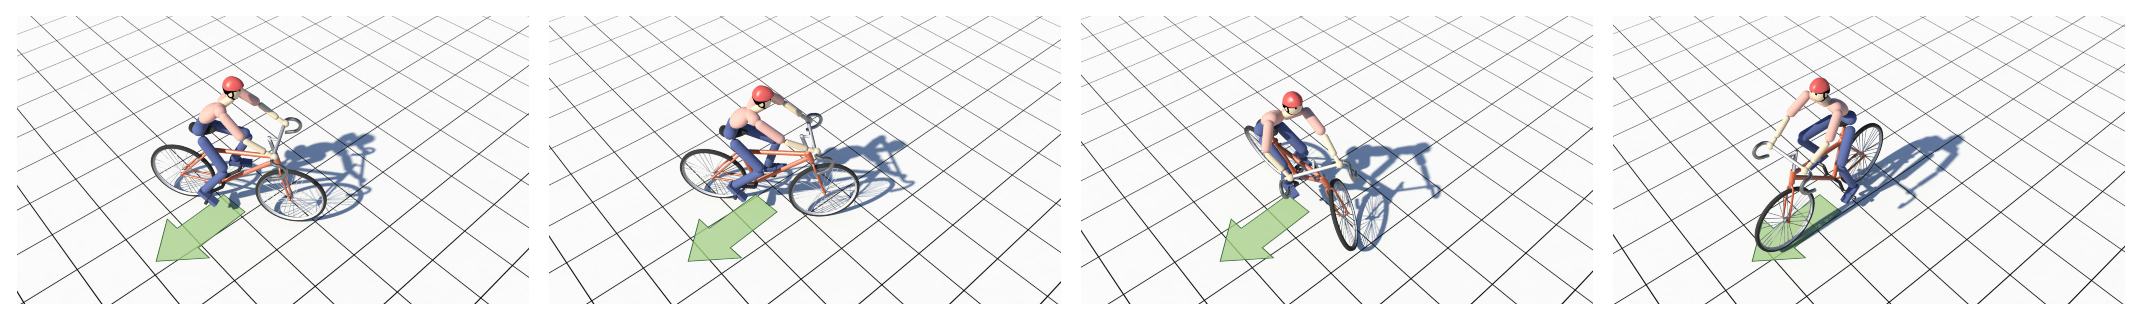
\includegraphics[width=\textwidth]{figures/maneuver}
\caption{A character steers the road bike towards the green arrow.}
\label{fig:balance}
\end{figure*}

\begin{figure*}[!t]
\centering

\includegraphics[width=\textwidth]{figures/staircase}
\caption{A character rides down a set of stairs without falling over.}
\label{fig:stair}
\end{figure*}


\begin{table}[!b]
\centering
\begin{tabular}{|l|c|c|}
\hline
task & states & actions \\
\hline
momentum-driven & & \\
\hline
going over curbs      & $t, \beta$   & $\dot{v}_r, \tilde{\phi}$\\
endo (lifting)        & $t, \beta$  & $\tau_f, \tilde{y}, \tilde{z}$ \\
front wheel pivot     & $t, \dot{\gamma}$ & $\dot{\theta}, \tau_f, \tilde{y}, \tilde{z}$\\
bunny hop             & $t, h_f, h_r$ & $\tilde{y}, \tilde{z}$\\
\hline
balance-driven & & \\
\hline
balance and steering  & $\theta, \Delta \theta, \alpha, \dot{\alpha}$ & $\dot{\theta}$ \\
wheelie               & $\alpha, \dot{\alpha}, \beta, \dot{\beta}, \Delta \beta, v_r, \psi, \dot{\psi}$  & $\dot{v}_r, \dot{\psi}$ \\
endo (balance)        & $\theta, \alpha, \dot{\alpha}, \beta, \dot{\beta}, \Delta \beta$ & $\dot{\theta}, \tau_f$ \\
back hop              & $\alpha, \dot{\alpha}, \beta, \dot{\beta}, \Delta \beta, x, y, z$ & $\dot{x}, \dot{y}, \dot{z}$\\
high wheeler (stunt)  & $\beta, \dot{\beta}, \Delta \beta, \Delta v_f$ & $\dot{v}_f$\\
unicycle              & $\alpha, \dot{\alpha}, \beta, \dot{\beta}, v_r, \Delta v_r, \chi$ & $\dot{v}_r, \dot{\chi}$\\
\hline
 \end{tabular}
 \caption{Choices of states and actions for each bicycle task. Note that in the momentum-driven tasks, the actions only depend on time $t$ while the remaining states are used to compute the reward. }
 \label{table:stateActions}
 \end{table}

\paragraph{Balance and steering.} Riding a bicycle requires balance and steering. Balance can be maintained by steering toward the falling direction, which generates centrifugal force to push the bike upright. Figure~\ref{fig:balance} shows that our learned controller enables the rider to balance and steer the bike towards a user-specified direction. The bike follows the green arrow closely even when the user changes the desired direction abruptly. This agile steering behavior is achieved through ``counter-steering'': a momentarily steering in the opposition direction to initiate a sharp turn~\cite{Rankine1870}, which emerged automatically from the policy search. We also tested the robustness of our balance and steering controller on a bumpy terrain, which is represented as a noisy height field sampled from a uniform distribution $h\sim U(0, 0.05)$ (unit: meter). Even though the bicycle jumps and the handlebar is perturbed constantly, the rider still manages to balance and closely follows the desired direction. In addition, the accompanying video shows an initial starting motion, in which the rider's left foot is scripted to push the ground and move towards the pedal. Based on this single trajectory of foot and the learned balance policy, we used IK to generate the full-body motion of the starting phase.

\paragraph{Going down stairs.} Figure~\ref{fig:stair} shows the character riding down a series of stairs. Each step is 0.15m high and 0.8m wide. We used the same balance controller as in the previous example. This balance task is more challenging because the frequent loss of contact and the sudden collisions between the front tire and the ground narrow the window of effective control and introduce large perturbations. Initially, the rider needs to make large corrections with the handlebar to keep balance when the forward speed is low. As the bicycle travels faster, the corrections become smaller and steadier.

\begin{figure*}[!t]
\centering

\includegraphics[width=\textwidth]{figures/Curb}
\caption{A character lifts the front wheel to ride over a curb.}
\label{fig:curb}
\end{figure*}

\begin{figure*}[!t]
\centering

\includegraphics[width=\textwidth]{figures/endo}
\caption{A character performs an endo and balance on the front wheel.}
\label{fig:endo}
\end{figure*}

\paragraph{Going over curbs.} Riding over curbs (Figure~\ref{fig:curb}) can be performed by lifting the front wheel using feed-forward control only. We therefore parameterized the actions with two splines (Table~\ref{table:stateActions}) and trained the controller using CMA. We used a task-specific reward function to maximize the pitch of the bicycle $R_t = \beta$ during lifting. In the animation, as the bicycle approaches a curb (0.12m high), the rider first leans forward and then pushes her upper body backwards. When the arms are stretched out to the maximum length, the sudden deceleration of the upper body pitches the whole bike upwards. The pitch angle is further increased by pedaling faster. This sequence of highly coordinated movements is discovered automatically by the policy search algorithm. Once the front wheel goes over the curb, the balance controller takes over and keeps the bike upright when the rear wheel hits the curb.

\paragraph{Real time user interaction.} A user can interact with our bike simulation in real time. We video captured a sequence that shows a person using a joystick that is equipped with motion sensors to control the rider and the bicycle. The rider goes over a curb, survives a crosswind, goes down a set of stairs, and follows a curvy path to the goal. Note that the user only gives high level commands such as the desired steering angle and the timing of lifting the front wheel. The balance, the actual steering and the rider's motions are all controlled by the policy learned from the offline training process.

\paragraph{Wheelie.} A wheelie is a stunt maneuver in which the rider first lifts the front wheel and maintains balance on only the rear wheel. Lifting the front wheel on a BMX bike is considerably easier than on a road bike due to the shorter distance between the wheels. It can be achieved by increasing the speed of pedaling without any noticeable upper body movements. For this reason, we used only a feedback controller (Table~\ref{table:stateActions}) to perform a wheelie, including both the initial lift and the later balance. Once the front wheel leaves the ground, the rider adjusts the forward speed to keep the desired pitch angle. He leans his upper body to the left or to the right to correct any lateral instability.

\paragraph{Endo.} Figure~\ref{fig:endo} shows an endo. In contrast to a wheelie, an endo lifts the rear wheel and balances on the front wheel. In spite of its symmetry to a wheelie, an endo requires an entirely different set of skills and environments. Endos are usually performed on a gentle downward slope, which provides the needed forward momentum when the driving wheel is off the ground. We used a slope of 2.5 degrees in our example. We first search for a feed-forward controller that maximizes the negative pitch angle $R_t = -\beta$ to initiate the stunt. The resulting controller slowly moves the rider's pelvis to the back, and then quickly throws it to the front to lift the rear wheel.

The feed-forward controller is succeeded by a feedback balance controller. To maintain an endo, the rider continuously applies or releases the front brake for longitudinal balance and steers the handlebar towards the direction of leaning for lateral balance. This stunt is especially challenging. If the pitch angle is too large, when the COM is above or in front of the front tire contact, such a gentle slope cannot provide enough acceleration to prevent overturning. If the pitch angle is too shallow, to prevent the rear wheel from dropping to the ground, braking hard will quickly halt the bicycle and make the balance strategy of ``steering toward falling'' ineffective. This complicated coupling between the pitch angle, the speed and the lateral balance makes heavy demands on the policy search algorithm. NEAT successfully finds a policy that can maintain balance for an extensively long period of time. Figure~\ref{fig:simpleNetwork} Right illustrates the complex neural network required for this task.

In the accompanying video, we also demonstrate the learning process of an endo. The animation shows the resulting balance controller after one, five and ten iterations. As more iterations are finished, the rider gradually masters an endo and maintains balance for a longer period of time.

\begin{figure*}[t]
\centering

\includegraphics[width=\textwidth]{figures/frontWheelPivot}
\caption{A character completes a quick 180-degree turn by pivoting the bicycle on the front wheel.}
\label{fig:pivot}
\end{figure*}


\begin{figure*}[t]
\centering
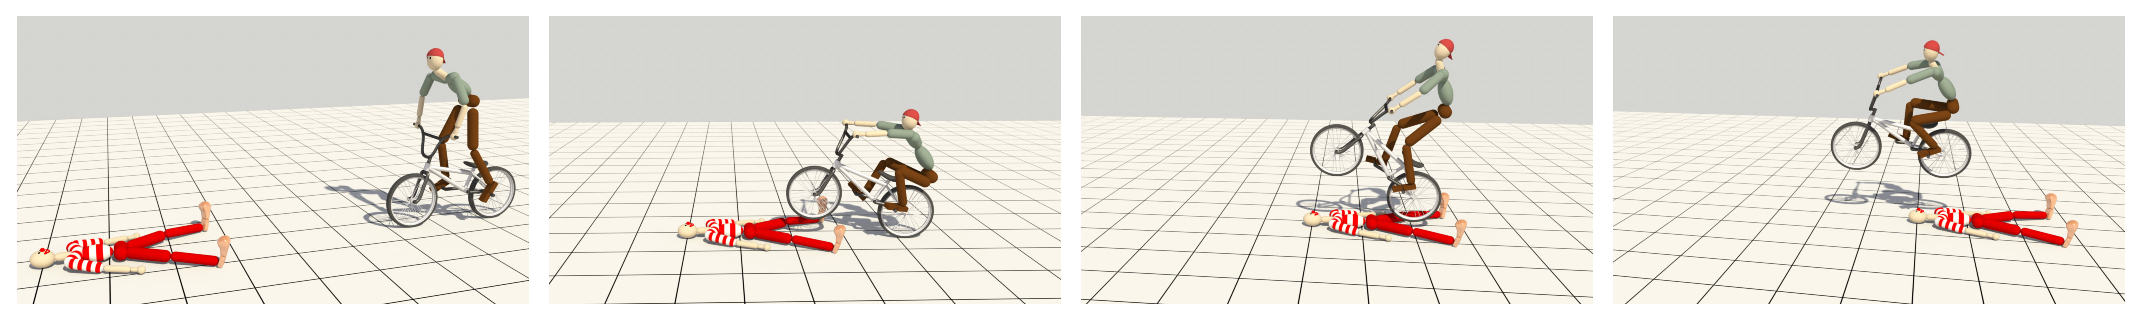
\includegraphics[width=\textwidth]{figures/bunnyHop}
\caption{A character performs the American bunny hop over a clown lying on the ground.}
\label{fig:bunnyhop}
\end{figure*}

\paragraph{Front wheel pivot.} A front wheel pivot (Figure~\ref{fig:pivot}) is a fast way to turn the bicycle 180 degrees by pivoting on the front wheel. We used a feed-forward controller and applied two separate task-specific rewards during two phases of this motion. The first reward function maximizes the angle of turning during the pivoting phase.
\begin {displaymath}
\begin{array}{ll}
R_{t_1} = & \left\{ \begin{array}{ll}
\dot{\gamma} \Delta t & \textrm{if }h_r > 0.01,\\
0 & \textrm{otherwise.}
\end{array} \right. \\
\end{array}
\end {displaymath}
After the rear wheel touches the ground, we switch to a learned balance controller and measure how long the bicycle can stay balanced: $R_{t_2}=1$ if the bicycle remains upright. Without the second reward function, the ``optimal'' policy can produce a large roll during the pivoting phase, after which the rider cannot recover balance. In the animation, the rider performs an endo after turning the handlebar sharply to the left. As a result, the rider and the bike pivot around the front wheel and the 180-degree turn finishes within three seconds.

\paragraph {Back hop.} The back hop is another way to balance on the rear wheel. This feedback balance strategy uses small hops to change the relative position between the contact and the COM. In the animation, the rider and the bike start at an initial pose in which the COM is behind the contact point between the rear wheel and the ground. The bike will fall backwards if the rider does not correct for this. He bends his knees and then extends them to bring the rear wheel off the ground. He quickly pulls the handlebar towards himself in mid-air to adjust the pitch of the bicycle. When the rear wheel lands, the COM comes closer to the ground contact position. As a result, the rider can continue to hop and balance for a long time.

\paragraph{Bunny hop.} Figure~\ref{fig:bunnyhop} shows the rider performing a bunny hop on a BMX bike. A bunny hop is a stunt where the rider jumps with the bike over an obstacle or a trench. The task-specific reward function for the feed-forward controller is evaluated based on the height of both tires above the ground $R_t=h_fh_r$. Right before the hop, the rider first leans forward and then moves his pelvis rapidly towards the back of the bicycle. This vigorous motion tilts the bicycle upward. The rider then jumps with the bicycle over a clown lying on the ground. We were pleased to see that the optimal policy for the bunny hop motion includes a phase that tilts the bicycle up, which is essential to jumping for a greater height and distance. This style is known as the ``American bunny hop''.

\begin{figure*}[t]
\centering

\includegraphics[width=\textwidth]{figures/velocipede}
\caption{A character rides a high wheeler and performs a stunt in which he rides backward on a single wheel.}
\label{fig:highwheeler}
\end{figure*}

\begin{figure*}[t]
\centering

\includegraphics[width=\textwidth]{figures/unicycle}
\caption{A clown rides a unicycle.}
\label{fig:unicycle}
\end{figure*}

\paragraph{Riding a high wheeler.} The peculiar design of a high wheeler makes ``headers'' a significant hazard, in which the rider gets pitch forward off the bicycle. We took on the challenge and designed a stunt that we had never seen performed on a high wheeler (Figure~\ref{fig:highwheeler}). During the stunt, the rider intentionally stops the bike to initiate a forward rotation. He then carefully changes pedaling speed to avoid taking a header and successfully rides backward on a single wheel. The rider can balance for a few seconds even without a lateral balance controller, probably due to the prominent gyroscopic effect from the large rotating front wheel. When the rider starts to lose balance, he accelerates to return to the normal riding mode, in which we used the same balance and steering controller as in the road bike examples.

\paragraph{Riding a unicycle.} The unicycle and the bicycle have many similarities. We have found that our algorithm is general enough to handle balance on a unicycle. Similar to some bicycle stunts, the longitudinal balance on a unicycle can be maintained via speeding-up or slowing-down, while the lateral balance can be maintained through steering toward falling. Unfortunately, unicycles do not have handlebars to steer. To steer the unicycle to the left, the rider needs to twist his upper body to the right. The unicycle will counter-rotate to the left due to the conservation of angular momentum. Figure~\ref{fig:unicycle} shows a clown riding a unicycle. To start riding, the clown first pedals backward, which leans the unicycle to the front. He then accelerates until the actual speed matches the user-specified desired speed. During riding, the clown repeatedly twists his waist to keep the lateral balance, which causes the unicycle to travel in a slightly sinusoidal path.



\section{Discussion}
\label{sec:Evaluation}

\begin{sidewaystable*}[ht]
\centering
\begin{tabular}{|l|c|c|c|c|c|c|c|c|c|}
\hline
task & wrist & elbow & scapula & shoulder & pelvis & hip & knee & ankle & ratio \\
\hline
\begin{tabular}{@{}l@{}}balance and \\steering (flat)\end{tabular} & 50 (5) & 150 (20) & 200 (30) & 550 (40) & 2000 (100) & 500 (150) & 500 (50) & 500 (50) & 0.9\\
\hline
unicycle & 10 (1) & 100 (5) & 100 (20) & 150 (10) & 2000 (30) & 100 (95) & 100 (90) & 60 (20) & 0.89\\
\hline
wheelie  & 10 (10) & 100 (30) & 100 (50) & 150 (80) & 2000 (100) & 500 (150) & 100 (100) & 60 (60) & 0.81\\
\hline
\begin{tabular}{@{}l@{}}going over \\curbs\end{tabular}& 50 (30) & 150 (50) & 200 (50) & 550 (80) & 2000 (100) & 500 (150) & 500 (100) & 500 (60) & 0.76\\
\hline
high wheeler & 50 (10) & 150 (50) & 200 (20) & 550 (200) & 2000 (300) & 500 (440) & 500 (360) & 500 (230) & 0.64\\
\hline
\begin{tabular}{@{}l@{}}balance and \\steering (bumpy)\end{tabular} & 50 (50) & 150 (100) & 200 (100) & 550 (350) & 2000 (400) & 500 (300) & 500 (350) & 500 (200) & 0.58\\
\hline
\begin{tabular}{@{}l@{}}front wheel \\pivot\end{tabular} & 250 (50) & 500 (150) & 500 (150) & 550 (400) & 2000 (600) & 500 (500) & 500 (280) & 500 (80) & 0.58\\
\hline
staircase & 50 (40) & 150 (100) & 200 (90) & 550 (350) & 2000 (400) & 500 (450) & 500 (450) & 500 (80) & 0.56 \\
\hline
bunny hop & 20 (15) & 50 (50) & 500 (150) & 550 (150) & 2000 (750) & 500 (400) & 500 (380) & 500 (220) & 0.44\\
\hline
endo & 50 (50) & 100 (100) & 100 (100) & 550 (400) & 2000 (600) & 500 (470) & 500 (485) & 500 (150) & 0.45\\
\hline
back hop & 250 (90) & 500 (400) & 500 (500) & 550 (545) & 2000 (900) & 500 (500) & 500 (450) & 500 (140) & 0.33\\
\hline
 \end{tabular}
 \caption{Torque limits (Unit: Nm) for different tasks. The values without the parenthesis are used for learning. The values within the parenthesis are the lowest torque limits that can be used in the simulation before the motion starts to fail. The amount of reduction is a measure of the robustness of the learned controllers. More reduction means a more robust controller. The last column reports the reduction ratios of average torque limits, which are sorted from high to low. This ranking is a possible indication of the difficulties (from low to high) that the learning algorithm think for each task. }
 \label{table:torqueLimit}
\end{sidewaystable*}


We have presented an algorithm for animating bicycle stunts.  Key aspects of our approach include a fast and stable physical simulation,
policy search for POMDP, and
the use of a sample-based optimization solver that searches for both the structure and the weights of a neural network.
Our system allows us to control a human character that
performs a variety of bicycle stunts, including wheelie, endo, bunny hop, front wheel pivot and back hop.
Our characters can learn to master the most demanding balance tasks in minutes, which challenges most people and takes months of practice to learn.

Although the learning algorithms presented in this chapter are general, the qualities of simulated motions vary with different tasks. We notice that some of the stunt motions do not look as compliant as those performed by real human riders due to three possible reasons. First, we chose large torque limits to allow robust control for various challenging maneuvers (Table~\ref{table:torqueLimit}). We used the same torque limits both in offline learning and online simulation to generate the results shown in the accompanying videos. To investigate whether we can achieve more compliant motions, we reduce the joint torque limits for simulation until the rider can no longer maintain balance (shown as the values in the parenthesis in Table~\ref{table:torqueLimit}). Although our controllers are robust when executed with smaller amount of torques, the resulting human motion appear very similar. The second possible reason is that we did not minimize rider's effort during offline learning. We found that it is difficult to weigh the effort minimization term because it competes with the task-specific objective. One possible solution is to implement prioritized optimization \cite{delasa:2009} to incorporate the effort minimization objectives. The last reason is probably due to the use of actuator constraints in ODE. The actuator constraints usually result in more stable simulation. However, since the joint torques are solved together with all other constraint forces, this allows the character to react instantaneously. We believe that the lack of reaction latency contributes to the stiffness of the motion. Using traditional PD servos could mitigate this problem but could also significantly increase the time of learning and simulation.

\begin{figure}[ht]
  \centering
  \includegraphics[width=5in]{figures/TorquePlot}
  \caption{Torque trajectories over time of performing an endo and riding a bicycle on a flat ground. }
  \label{fig:torquePlot}
\end{figure}

We further examine the torque trajectories (Figure~\ref{fig:torquePlot}), and observe that the controllers learned different strategies to achieve different tasks. In the endo example, the torques switch abruptly between the two extreme values. It is similar to the ``bang-bang control'' that frequently arises in time-critical tasks, indicating that the task of endo might also be time-critical. In contrast, the torque trajectory of riding a bicycle on a flat terrain shows more smooth transitions, which implies that normal biking does not require instant reactions and is thus an easier task.

Policy search is a powerful method for learning optimal controllers. However, manually designing parametrization of the policies could be challenging for difficult tasks. Combining policy search with NEAT makes it easy to use and unleashes its full power. We have demonstrated that searching for both the parametrization and the parameters of a policy creates robust controllers for a wide variety of bicycle balance tasks. Since many previous studies focused on optimizing the parameters alone, we evaluated the necessity of optimizing the parametrization. Figure~\ref{fig:compare} Left and Right compares two policy search results with a fixed and with an evolving parametrization for the balance task of an endo. Both searches started with the same parametrization: a neural network with direct connections between the input and the output layers. We used CMA to search for only the weights while we used NEAT to evolve both the weights and the network structure. Both algorithms were run for 50 iterations with 90 samples per iteration. We ran each search ten times with different random seeds to reduce the stochastic bias. Figure~\ref{fig:compare} Left plots the curves of the policy value versus the number of iterations in the CMA search. Note that none of the searches reached a value of 3000. In comparison, eight out of ten NEAT searches found policies scored higher than 3000 (Figure ~\ref{fig:compare} Right). Three of them reached almost 7000. The average final policy value of NEAT was almost twice its CMA counterpart. A similar comparison was conducted between neuroevolution with and without augmenting topology, and this told the same story (Figure~\ref{fig:compare} Middle vs. Right). Even though we only reported the detailed comparison for this particular example, we observed the same trend for other bicycle stunts: policy search with an evolving parametrization significantly outperforms search with a fixed parametrization. The neural network structure for all the balance-driven tasks are shown in Appendix \ref{chapter:AppendixC}.

\begin{figure*}[ht]
  \centering
  \includegraphics[width=\textwidth]{figures/NeatCMAComp}
  \caption{A comparison between policy searches with a fixed and an evolving parametrization. Left: The policy value vs. the number of iterations for ten policy searches on a fixed parametrization using CMA. Middle: Results of ten policy searches on a fixed parametrization using neuroevolution without augmenting topology. Right: Results of ten policy searches on an evolving parametrization using NEAT. }
  \label{fig:compare}
\end{figure*}

As illustrated in Chapter \ref{sec:results}, many bicycle stunts need balance in both the longitudinal and lateral directions. In our implementation, we decoupled the balance task in these two directions and learned the task in two steps. In the first step, we focused on longitudinal balance and chose only the relevant states and actions. We artificially increased the width of the tire to 20cm so that the controller did not need to be concerned about the loss of balance in the lateral direction. This is analogous to using training wheels in real life. Once the longitudinal controller had been learned, we fixed that part of the neural network, reduced the width of the tire back to normal\footnote{The tire width of the road bike and the high wheeler is 1.5cm while the tire width of the BMX bike and the unicycle is 3cm.} and then performed the second step of training for lateral balance. Although in theory, optimizing a controller for the longitudinal and the lateral balance simultaneously would have a better global optimum, in practice, searching for a policy in a higher dimensional space is subject to local minima and thus could produce inferior results. In all our examples, this two-step training found better policies than training both longitudinal and lateral balance simultaneously.

\newtext{Although we chose to use neural network and NEAT to tackle this problem, there could be other althernatives. One possibility is to use optimal control algorithms, such as Linear Quadratic Regulator (LQR) or Dynamic Differential Programming (DDP). These methods start with a nominal trajectory and linearize the dynamics around it. However, it is not clear to us how to design good nominal trajectories for a wide variety of challenging bicycle stunts. Moreover, bicycle stunts involve frequent contact changes. This makes the dynamics nonlinear and discontinuous. Thus, using linearized dynamics is unlikely to succeed. We have also tried a couple of other reinforcement learning techniques. They ended up unsuccessful, but these valuable experience has led us to our current solution. Our first attempt was to use standard value iteration method with a discretized state space. The high dimensional state space made the tabular representation infeasible. We encountered the convergence issue when the state space was parameterized by polynomial and Gaussian kernel bases. We also experimented with a few model-free learning algorithms. For example, SARSA($\lambda$) demonstrated some potential (\ie the normal cycling was successful), but the computation time was too long even for the simplest task. Although our final decision was to use policy search, the initial experiments were unsuccessful due to an overly simplified policy parametrization: a neural network without hidden layers. Using quadratic features to enrich the inputs of the network, we had some limited success with the optimal solutions solved by CMA. However, without a systematic way to perform feature selection, the likelihood of finding a successful local minimum is low due to the large number of quadratic features. Finally, we chose NEAT, a bottom-up approach that complexifies the parametrization from the simple network. This method consistently found policies that worked for all our examples.}

NEAT provides an effective way to search for both the parametrization and the parameters, which frees us from laborious and unintuitive manual tuning of the network structure. However, to formulate an MDP, we still need to design the state space, the action space and the reward function. \del{While designing the state space is often straightforward, choosing appropriate actions for a specific task requires domain knowledge.} \newtext{Selecting the right features to represent the states and the actions is vital to the success of the entire algorithm. The rule of thumb is to choose only a small number of features that are most relevant to the task. If too many states and actions are used (\eg all the simulation states as the state space and all the joint torques as the action space), it is not likely that NEAT will find a successful controller due to the high dimensional search space. Selecting the states and actions for a specific task often requires domain knowledge. For example, knowing how to steer a unicycle (twisting the upper body) is essential for the unicycle balance task.} Likewise, designing a good reward function requires some trial-and-error experiments. Our reward functions initially contained only the task-specific terms. We found that the algorithm often discovered a policy that had a high value but resulted in undesired motions: The rider performed redundant movements as long as this did not affect the balance. We eliminated these undesired motions by adding regularization terms to the reward function. However, selecting states, actions and reward functions is unavoidable when formulating and solving MDPs. Inverse reinforcement learning \cite{Ng:2000} might be a promising approach, but this requires data generated from the optimal policy, such as motion capture data from real stunt bikers. \newtext{Another promising future research is to automatically extract features for different bicycle stunts using deep learning. Please refer to Chapter \ref{sec:future} for more discussion on this topic. }\del{Compared to manually designing a policy parametrization, learning the domain knowledge and tuning the reward function is more intuitive and fun.}

Our system has a few limitations. We used ball joints to attach the feet to the pedals. These bilateral joint constraints simplify the simulation but render some motions less realistic: The brief moment in our bunny hop animation when the rear wheel pops off the ground just before the hop typically is not seen in the real stunt. Faithfully modeling the contact between the feet and the pedals could solve this problem. However, this will make the simulation more expensive and the learning more difficult. In the learning, we separated the feed-forward and feedback controllers. This treatment works well if the feed-forward controller is applied for a short period and then we switch to the feedback controller. However, in a real-life performance, stunt bikers exhibit both feed-forward and feedback controls at the same time, which allows them to perform longer and more difficult stunts. This might be one of the reasons that our algorithm cannot generate a 360-degree front wheel pivot. Our interactive simulation does not allow the user to arbitrarily concatenate the stunts. Successful stunts demand a stable initial pose, appropriate speed and sometimes a favorable terrain. All these requirements together prevents us from concatenating stunt controllers arbitrarily. Learning additional intermediate controllers between stunts might be a possible solution.

There are a number of interesting avenues for future work.  We believe that our algorithm will not be limited to the bicycle control tasks. It has the potential to solve other challenging control problems, such as gymnastics, skateboarding, surfing and dancing. Deep learning \cite{Hinton:2007} and deeper neural networks could be explored for even more difficult stunts. Our work has concentrated on controllers for individual stunts. It would be interesting to investigate a sequence of stunts that traverse a bicycle course with obstacles. Finally, it would be fascinating to manufacture a mini bicycle and a robotic rider and apply our controllers to make them perform stunts in the real world.

\chapter{Conslusion and Future Work}

\section{Conclusion}
In this disseration, we have presented a principle way to synthesize locomotion of humans and animals. Our algorithms can control characters of different morphologies to move efficiently and robustly in complex physically-simulated environments and to achieve challenging tasks. The key components of our algorithms are a set of powerful computational tools, including physical simulation and controller optimization. Although combining simulation and optimization is not a novel idea in motion synthesis, in contrast to the prior work, we examine and identify those commonly-used simplifications that can affect the quality of the motions. We eliminate these simplifications by designing new simulation and optimization techniques. Our simulators are faster, more stable and more accurate. Our optimizator can search a higher-dimensional space with both continuous and discrete variables, which may lead to better optimal solutions. These computational tools make it possible to study a more diverse set of motions in nature than were previous possible in the character animation literature.

Chapter 3 described computational tools to study the diversity of swimming motions for aquatic creatures with different body shapes. This is made possible by an accurate swimming simulation and a powerful evoluationary optimization. Compared to the simplified fluid model, our swimming simulation solves the Navier-Stokes equations. It can capture important features of water, including incompressibility and vortices, that affect swimming strategies. In contrast to the traditional alternating two-way coupling technique, our simulation solves the dynamic equations of fluids and articulated rigid bodies simultaneously. This increases the numerical stability and drastically speed up the computation. Simulating the hydrodynamic environment with Navier-Stokes equations introduce new challenges to the classical optimization algorithms. We demonstrated that CMA works well in this scenario. As a result, our algorithms can discover the most efficient swimming gait for a given creature autonumous, without any human intervention. Our results showed that the synthesized swimming motions agree well with those employed by real aquatic animals.

Chapter 4 presented computational tools to study locomotion of soft body characters without skeleton support. We developed a muscle model that worked seamlessly with the state-of-the-art FEM simulation for soft materials. This muscle model is inspired by muscle structures found in real soft body animals. It lowers the dimensionality of the control space and ensures that the overall motion is coordinated. We demonstrated how to use finite-horizon trajectory optimization to control the locomotion. The key to our success is to identify that the widely-used simplification that separates contact planning with controller optimization is not good enough to achieve a stable locomotion. To solve this problem, we formulated a QPCC and developed an efficient solver. Consequently, effecitve control strategies and natural locomotion emerge autonumously from the optimization solution.

Chapter 5 demonstrated computational tools to study agile human motions on a bicycle. We developed the first reinforcement learning algorithm that allows a virtual human character to learn bicycle stunts in a physically simulated environment. The algorithm is so efficient that most of stunt actions are learned in hours, which is even faster than the best human stunt bikers. An important lesson we have learned in this work is that it is difficult to design a good controller parametrization manually, especially for challenging locomotion tasks. The common practice of using a fixed policy parameterization tuned by users can severely limit the power of policy search algorithms. We eliminated this restriction by using NEAT, an algorithm that can simulnaneously optimize both the parametrization and the parameters of a neural network. Eventually, the virtual character learned to perform a wide variety of stunts automatically, without the tedious manual tuning of controller parametrizations.

Chapter 6 explored an efficient method to develop humanoid robot controllers for the tasks of rising from a leaning/sitting/kneeling position to an erect stance. We built an accurate physical simulation, optimized controllers in the simulation and transfered the controller to a real robot. We investigated several factors that lead to the reality gap and demonstrated in several cases that this gap may be crossed with an improved physical simulation. We perform iterative simulation calibration using data collected from robot experiments. After a small number of iterations, the controller designed in a simulation can be successfully transferred to the robot. This work shows that it is possible to apply the computational tools that were developed for character animations to design robotic controllers. It is an important milestone towards a fully automatic computational framework that can design the next-gen robots with extensive agility and maneuverability.

\section{Future Work}

The work presented in this dissertation opens the door to many promising directions for future work. One interesting direction is to study swimming motions of soft body animals. Studying soft body locomotion in water may have more foundamental impacts than articulated swimming creatures (Chapter 3) or soft body locomotion on land (Chapter 4). Most of the soft body animals on our planet, such as squid, octopus, seaslug and jellyfish, reside in oceans and they present more diversity in terms of swimming gaits. Their flexible body shapes could enable more efficient propulsion mechansims than those of animals with rigid skeletons. For example, a jellyfish was found as ocean's most efficient swimmer \cite{Gemmell:2013}. In addition, the surface of aquatic animals with skeletons is still highly deformable due to the presence of skins, ligament and muscles. It is more appropriate to model them as soft bodies rather than as articulated rigid bodies, as we did in Chapter 3. I believe that it would be promising to combine the approaches in Chapter 3 and 4 to synthesize swimming motions for soft body characters.

Another important future work is to use deep neural networks in reinforcement learning. Although NEAT frees us from laborious manual tuning of neural network structure in Chapter 5, we still need to specify the state and the action space for each task. For example, to keep balance on a bicycle, states should include the center of mass or the bicycle leaning angle. However, they may not carry over to a different task. Manually designing states and actions would not scale to more sophisticated characters, more complicated environments, or more challenging tasks. The way that we use these hand-engineered states and actions in reinforcement learning today is analogue to using HoG and SIFT features in computer vision a few years back. Recent advance in computer vision has shown promising results, which use deep neural networks, such as autoencoder \cite{Vincent:2008} or Restricted Boltzmann machine \cite{Hinton:2012}, to learn features automatically. I believe an important next step for character control is to employ similar techniques to discover important features.

A lot more work need be done in the future to transfer controllers from the simulation to the real world. Chapter 6 is an important step towards a fully automatic computational framework to design robotic controllers. Although it has shown promising results, we have not yet put it into a comprehensive test with more challenging tasks. One possible stress test is to use this method to transfer bicycle stunt controllers developed in Chapter 5 to a real robot. No matter whether the real robot can successfully perform bicycle stunts, it will provide us more insights about the causes of the reality gap and help us to eventually cross it.

\ignorethis{In my point of view, the most efficient way to design robotic controllers is to a two-step process. First, optimize the controller in a simulation, and second, transfer the controller to the real robot. We have done an excellent job in character animation for the first step. Through Chapter 3 to Chapter 5, we have demonstrated}


\begin{postliminary}
\references
\end{postliminary}
\end{document}
